\documentclass[10pt]{report}
\usepackage[margin=1in]{geometry} 
%\usepackage[margin=1.875in]{geometry} 
\usepackage{amsmath,amsthm,amssymb,amsfonts}
\usepackage{physics}
\usepackage{graphicx}
\usepackage{import}
\usepackage[width=0.8\textwidth]{caption}
\usepackage{subcaption}
\usepackage[subpreambles=true]{standalone}
\usepackage[square,sort,comma,numbers]{natbib}
\usepackage{hyperref}
\usepackage{scalerel}

\hypersetup{ %using this to remove ugly red square boxes around links
    colorlinks,
    linkcolor={red!50!black},
    citecolor={blue!50!black},
    urlcolor={blue!80!black}
}

%%%%%%%%%%%%%%%%%%%%%%%%%%%%%%%%%%%%%%%% used for code listings

\usepackage{color}
\definecolor{bluekeywords}{rgb}{0.13,0.13,1}
\definecolor{greencomments}{rgb}{0,0.5,0}
\definecolor{redstrings}{rgb}{0.9,0,0}

\usepackage{listings}
\lstset{language=[Sharp]C,
    showspaces=false,
    showtabs=false,
    breaklines=true,
    showstringspaces=false,
    breakatwhitespace=true,
    escapeinside={(*@}{@*)},
    commentstyle=\color{greencomments},
    keywordstyle=\color{bluekeywords}\bfseries,
    stringstyle=\color{redstrings},
    basicstyle=\footnotesize \ttfamily,
    numbers=left,
    frame=tb
}


%%%%%%%%%%%%%%%%%%%%%%%%%%%%%%%%%%%%%%%%
\usepackage{xargs}                      % Use more than one optional parameter in a new commands
\usepackage[pdftex,dvipsnames]{xcolor}  % Coloured text etc.
% 
\usepackage[colorinlistoftodos,prependcaption,textsize=normalsize, textwidth=2cm]{todonotes}
\newcommandx{\unsure}[2][1=]{\todo[linecolor=red,backgroundcolor=red!25,bordercolor=red,#1]{#2}}

\newcommandx{\note}[2][1=]{\todo[linecolor=black,backgroundcolor=yellow!40,bordercolor=black,#1]{#2}}
\newcommandx{\change}[2][1=]{\todo[linecolor=blue,backgroundcolor=blue!25,bordercolor=blue,#1]{#2}}
\newcommandx{\info}[2][1=]{\todo[linecolor=OliveGreen,backgroundcolor=OliveGreen!25,bordercolor=OliveGreen,#1]{#2}}
\newcommandx{\improvement}[2][1=]{\todo[linecolor=Plum,backgroundcolor=Plum!25,bordercolor=Plum,#1]{#2}}
\newcommandx{\thiswillnotshow}[2][1=]{\todo[disable,#1]{#2}}
%%%%%%%%%%%%%%%%%%%%%%%%%%%%%%%%%%%%%%%%%

\usepackage{setspace} % used for linespacing 


\numberwithin{equation}{chapter}

%\includeonly{chapters/chapter3}
%\includeonly{chapters/RiscVReferenceCard}


\begin{document}
    \pagenumbering{roman}
    \listoftodos[Notes]
    \newpage
    \title{Implementation of RISC-V in SME}
\author{Daniel Ramyar}
\maketitle
    \tableofcontents
    \clearpage
    \pagenumbering{arabic}
    \begin{onehalfspacing}
        \large
        \chapter{Introduction}
    In the modern age, computers have accelerated the scientific process many fold. Applications ranging from advanced weather models, the study of molecules to creating artificial intelligence has now become possible due to the rapid progress of computational power.
    
    Since the 1980s the computer architecture \texttt{x86}, pioneered by Intel, has been the de facto standard. 
    Ever since its inception, an average of 1 instruction has been added to the \texttt{x86} standard per week, resulting in over fifteen hundred \texttt{x86} instructions today\footnote{They can be found here \url{https://software.intel.com/en-us/articles/intel-sdm}}. This kind of bloat leads to inefficiency and needless complexity.
    
    This was not helped by the rapid advance in the miniaturization of transistors leading to huge leaps in computational power year over year making the mentioned deficiencies in the \texttt{x86} less relevant. The deficiencies are however beginning to show today, since we are nearing the end of moore’s law and we are no longer seeing leaps in computational power motivating us to rethink the \texttt{x86} architecture.
    
    Using the power of hindsight the \textit{Reduced Instruction Set Computing Five} or \textit{RISC-V} was created. The core of RISC-V consists of less than fifty locked down instructions and since RISC-V is open source, any additional custom instruction can be added.
    
    
    These days most measurement instruments are based on \texttt{x86} CPUs, which greatly limits the bandwidth at which data collection is possible and greatly limits the possibility for custom solutions, since the \texttt{x86} is a proprietary architecture owned by Intel. 
    
    For the aforementioned reasons, the RISC-V processor is especially well suited for embedding in scientific instruments and measuring devices and as such will play a central role in future physics instruments.
    Therefore a custom implementation of the RISC-V architecture for scientific purposes show great promise. 
    
    In this project we will design a RISC-V processor and implement it using Synchronous Message Exchange (SME), which is used to rapidly develop circuits for Field Programmable Gate Arrays (FPGAs).
        \chapter{Logic Design}
    
    This chapter aims to introduce the reader to the basics of logic design, which will be imperative to the understanding the subsequent chapters. The general structure of this chapter will be based on Appendix A in \cite{riscVbook}. 
    
    We will begin in Section \ref{section:Boolean_algebra} by introducing the fundamental algebra and the physical building blocks, used to implement the algebra, such as the OR gate. 
    
    Hereafter we will be using these building blocks to design and create the core components used in the RISC-V architecture such as the decoder and multiplexer in section \ref{section:Combinational_logic}. 

    \section{Boolean algebra}\label{section:Boolean_algebra}
    
        The fundamental tool used in logic design is a branch of mathematical logic called Boolean algebra. Compared to elementary algebra, where we deal with variables which represents some real or complex number, in Boolean algebra the variables are viewed as statements or propositions, which are either \textit{true} or \textit{false}.
        
        In addition to the variables in elementary algebra we also had a means of manipulating them. These manipulations are called operations which operates on the variables (operands) where the basic operators of algebra consists of $+$, $-$, $\cross$ and $\divisionsymbol$.
        
        In Boolean algebra we have a distinction between operators which work on one operand and the ones that work on to two operands. These are called unary and binary operators respectively. We will go through a description of these in the following section. 
        
        \subsection{Unary operators}\improvement{make ven diagrams to show the operator function}
        
            With a single binary operand p we have 2 possible input $true$ and $false$. All output combinations are summarized in Table \ref{LogicTable:unary}. Each numbered column here represents an unnamed operator. We will go ahead and describe one of these in the following. The rest can referred to in Appendix \ref{appendix:Unary_Operators}. 
            
            \begin{table}[h!]
                \centering
                \begin{tabular}{|c||c|c|c|c|}
                	\hline
                	  $p$   &   1    &    2    &    3    & 4       \\ \hline
                	$true$  & $true$ & $true$  & $false$ & $false$ \\ \hline
                	$false$ & $true$ & $false$ & $true$  & $false$ \\ \hline
                \end{tabular}
                \caption{Logic table of possible unary operators. Each numbered column represents an unnamed operator.}
                \label{LogicTable:unary}
            \end{table} 
        
            \subsubsection{Logical complement}
            
                For our first basic Boolean operator we have the logical complement operator, which is represented by NOT, !, $\neg$ or $\bar{x}$ in various literature and commonly referred to as the negation operator. 
                
                The negation operator inverts an operand such that $\neg true = false$ and $\neg false = true$.
                Using a table we can neatly represent the complete function of the negation operator. These tables are called \textit{logic tables}.
                
                A logic table has been created for the negation operator as can be seen in Table \ref{LogicTable:Negation}.  The first column represents our proposition and all its possible arguments $true$ and $false$. The second column is then the negated proposition.
                
                \begin{table}[h!]
                    \centering
                    \begin{tabular}{|c|c|}
                    	\hline
                    	  $p$   & $\neg{p}$ \\ \hline
                    	$true$  &  $false$  \\ \hline
                    	$false$ &  $true$   \\ \hline
                    \end{tabular}
                    \caption{Logic table of the negation operator where the proposition p, which is either true or false, can be found in the first column. In the second column we find $\neg p$, which is read as NOT $p$, and its return values.}
                    \label{LogicTable:Negation}
                \end{table}
            
            \subsubsection{Summary}
                
                We can now go ahead and fill the numbered columns Table \ref{LogicTable:unary} with the corresponding operators, which we have defined throughout this section and Appendix \ref{appendix:Unary_Operators}. The filled table can be found in Table \ref{LogicTable:unaryfilled}.
                
                \begin{table}[h!]
                    \centering
                    \begin{tabular}{|c||c|c|c|c|}
                    	\hline
                    	  $p$   & $T(p)$ & $I(p)$  & $\neg p$ & $F(p)$  \\ \hline
                    	$true$  & $true$ & $true$  & $false$  & $false$ \\ \hline
                    	$false$ & $true$ & $false$ &  $true$  & $false$ \\ \hline
                    \end{tabular}
                    \caption{Logic table of possible unary operators where $p$ is our proposition. Column 2-5 shows the output of the corresponding operator.}
                    \label{LogicTable:unaryfilled}
                \end{table} 
                
                 
\newpage        
        \subsection{Binary operators and disjunctive normal form}\label{DNF}
        
            With two binary operands, $p$ and $q$, there exist four possible combinations between their respectable values namely $(true, true)$, $(true, false)$, $(false, true)$, $(false, false)$.
            
            Compared to the previous section we now have 4 possible input values for our yet unnamed operators $X(p, q)$. There exist 16 unique sets of outputs and therefore 16 possible operators. An example of a set of outputs could be 
            \begin{equation}
                X(p, q) =\{true, false, false, false\}
            \end{equation}
            where $(p, q) = \{(true, true), (true, false), (false, true), (false, false)\}$ is the set of possible inputs. 
            
            All output sets are summarized in Table \ref{LogicTable:PossibleOperators} where each numbered column represents an unnamed operator. 
            
            We will in this section start by defining the basic operators from which we will derive the rest. For brevity we will only go through the 3 most commonly used operators, the rest can be referred to in Appendix \ref{appendix:Binaray_Operators}.  
            
            The choice of basic operators is arbitrary but I have chosen the operators for which it is the easiest to derive all other operators, since there exists a method to convert any truth table into a Boolean expression using these which we will get into later.
             
            
            \begin{table}[h!]
                \centering
                \begin{tabular}{|c|c||c|c|c|c|c|c|c|c|c|c|c|c|c|c|c|c|}
                	\hline
                	$p$ & $q$ &  1  &  2  &  3  &  4  &  5  &  6  &  7  &  8  &  9  & 10  & 11  & 12  & 13  & 14  & 15  & 16  \\ \hline
                	$t$ & $t$ & $t$ & $t$ & $t$ & $t$ & $f$ & $t$ & $f$ & $f$ & $t$ & $t$ & $f$ & $t$ & $f$ & $f$ & $f$ & $f$ \\ \hline
                	$t$ & $f$ & $t$ & $t$ & $t$ & $f$ & $t$ & $t$ & $t$ & $f$ & $f$ & $f$ & $t$ & $f$ & $t$ & $f$ & $f$ & $f$ \\ \hline
                	$f$ & $t$ & $t$ & $t$ & $f$ & $t$ & $t$ & $f$ & $t$ & $t$ & $f$ & $t$ & $f$ & $f$ & $f$ & $t$ & $f$ & $f$ \\ \hline
                	$f$ & $f$ & $t$ & $f$ & $t$ & $t$ & $t$ & $f$ & $f$ & $t$ & $t$ & $f$ & $t$ & $f$ & $f$ & $f$ & $t$ & $f$ \\ \hline
                \end{tabular} 
                \caption{Logic table of possible binary operators where $t=true$ and $f=false$. Each numbered column represents an unnamed operator.}
                \label{LogicTable:PossibleOperators}
            \end{table}
        
            \subsubsection{Logical conjunction}
        
                The logical conjunction operator is represented by $\wedge$ in mathematics; AND, \&, \&\& in computer science and a $\cdot$ in electronic engineering and commonly referred to as the AND operator or the logical product. The AND operator only results in a true value if both of the operands are true.
                
                Using Table \ref{LogicTable:PossibleOperators} we see that the set of outputs which corresponds to this definition is column 12 and is summarized in Table \ref{LogicTable:AND}. 
                
                Here we have the propositions $p$ and $q$ in the first two columns and all possible permutations between them in the following rows. The last column then shows the resulting value after doing the AND operation between $p$ and $q$. 
                
                \begin{table}[h!]
                    \centering
                    \begin{tabular}{|c|c|c|}
                    	\hline
                    	  $p$   &   $q$   & $p \wedge q$ \\ \hline
                    	$true$  & $true$  &    $true$    \\ \hline
                    	$true$  & $false$ &   $false$    \\ \hline
                    	$false$ & $true$  &   $false$    \\ \hline
                    	$false$ & $false$ &   $false$    \\ \hline
                    \end{tabular}
                    \caption{Logic table of the AND operator where $p$ is the first proposition and $q$ is the second. All possible permutations are then specified in each row for each proposition. The third column then shows the resulting value of the AND operation between $p$ and $q$.}
                    \label{LogicTable:AND}
                \end{table}
            
            \subsubsection{Logical disjunction}
            
                The logical disjunction operator is represented by $\vee$ in mathematics; OR, $\vert$, $\vert \vert$  in computer science and a $+$ in electronic engineering and commonly referred to as the OR operator or the logical sum. The OR operator results in a true value if one or more of the operands are true.
                
                Using Table \ref{LogicTable:PossibleOperators} we see that the set of outputs which corresponds to this definition is column 2 and is summarized in Table \ref{LogicTable:OR}. 
                
                Here we have the propositions $p$ and $q$ in the first two columns and all possible permutations between them in the following rows. The last column then shows the resulting value after doing the OR operation between $p$ and $q$.
                
                \begin{table}[h!]
                    \centering
                    \begin{tabular}{|c|c|c|}
                    	\hline
                    	  $p$   &   $q$   & $p \vee q$ \\ \hline
                    	$true$  & $true$  &   $true$   \\ \hline
                    	$true$  & $false$ &   $true$   \\ \hline
                    	$false$ & $true$  &   $true$   \\ \hline
                    	$false$ & $false$ &  $false$   \\ \hline
                    \end{tabular}
                    \caption{Logic table of the OR operator where $p$ is the first proposition and $q$ is the second. All possible permutations are then specified in each row for each proposition. The third column then shows the resulting value of the OR operation between $p$ and $q$.}
                    \label{LogicTable:OR}
                \end{table}
            
                We choose AND, OR and NOT to form our basic or primitive operators from which we will derive all remaining operators.
                
            \subsubsection{Exclusive disjunction and disjunctive normal form}
                
                The exclusive disjunction is represented by $\veebar$ in mathematics or XOR, \textsuperscript{$\wedge$} in computer science and commonly referred to as the XOR or exclusive OR operator. The XOR operator results in a true value only if the operands differ.
                
                Using Table \ref{LogicTable:PossibleOperators} we see that the set of outputs which corresponds to this definition is column 7 and is summarized in Table \ref{LogicTable:XOR}.
                
                Here we have the propositions $p$ and $q$ in the first two columns and all possible permutations between them in the following rows. The last column then shows the resulting value after doing the XOR operation between $p$ and $q$.
                
                \begin{table}[h!]
                    \centering
                    \begin{tabular}{|c|c|c|}
                    	\hline
                    	  $p$   &   $q$   & $p \veebar q$ \\ \hline
                    	$true$  & $true$  &    $false$    \\ \hline
                    	$true$  & $false$ &    $true$     \\ \hline
                    	$false$ & $true$  &    $true$     \\ \hline
                    	$false$ & $false$ &    $false$    \\ \hline
                    \end{tabular}
                    \caption{Logic table of the XOR operator where $p$ is the first proposition and $q$ is the second. All possible permutations are then specified in each row for each proposition. The third column then shows the resulting value of the XOR operation between $p$ and $q$.}
                    \label{LogicTable:XOR}
                \end{table}
            
                We can define this operator in \textit{disjunctive normal form} (DNF) or \textit{Sum of products form}, using our basic operators AND, OR and NOT. A logic equation (see section \ref{Section:BooleanEquation}) is said to be in DNF, when it consists of disjunctions between one or more conjunctions, where each of the propositions can be complemented.
                
                To write our operator in DNF, we first identify all true outputs in \ref{LogicTable:XOR} namely row 3 and 4. We then take a look at the corresponding input values
                \begin{equation}
                    (p,q) = (true, false) \quad \text{and} \quad (p,q) = (false, true)
                \end{equation}
                and applying the NOT operator on all the false values. We now have the two tuples
                \begin{equation}
                    (p,\neg q) = (true, \neg false) \quad \text{and} \quad (\neg p, q) = (\neg false, true).
                \end{equation}
                
                Hereafter we apply the AND operator between the values in each tuple of input such that
                \begin{equation}
                    p \wedge \neg q = true \wedge \neg false \quad \text{and} \quad \neg p \wedge q = \neg false \wedge true.
                \end{equation}
                Lastly we apply the OR operators between each tuple and we have the final expression for XOR in terms of the basic operators
                \begin{equation}
                    p \veebar q = (p \wedge \neg q) \vee (\neg p \wedge q).
                \end{equation}
                
                The procedure is summarized as follows
                \begin{enumerate}
                    \item Find all output values, which are true.
                    \item Negate all false input for corresponding true output value.
                    \item Apply AND operator between each value in each input tuple.
                    \item Lastly apply OR operator between each input tuple.
                \end{enumerate}
                Using this procedure any logic table can be expressed as a Boolean expression and will be used extensively throughout this thesis.
                
                
            \subsubsection{Summary}
            
                We can now go ahead and fill the numbered columns in Table \ref{LogicTable:PossibleOperators} with the corresponding operators, which we have defined throughout this section and Appendix \ref{appendix:Binaray_Operators}. The filled table can be found in Table \ref{LogicTable:BinaryOperators}. 
                
                \begin{table}[h!]
                    \centering
                    \begin{tabular}{|c|c||c|c|c|c|c|c|c|c|c|c|c|c|c|c|c|c|}
                    	\hline
                    	$p$ & $q$ & $\top$ & $\vee$ & $\leftarrow$ & $\rightarrow$ & $\uparrow$ & $P(p,q)$ & $\veebar$ & $\neg P(p,q)$ & $\leftrightarrow$ & $Q(p, q)$ & $\neg Q(p,q)$ & $\wedge$ & $\not\rightarrow$ & $\not\leftarrow$ & $\downarrow$ & $\bot$ \\ \hline
                    	$t$ & $t$ &  $t$   &  $t$   &     $t$      &      $t$      &    $f$     &   $t$    &    $f$    &      $f$      &        $t$        &    $t$    &      $f$      &   $t$    &        $f$        &       $f$        &     $f$      &  $f$   \\ \hline
                    	$t$ & $f$ &  $t$   &  $t$   &     $t$      &      $f$      &    $t$     &   $t$    &    $t$    &      $f$      &        $f$        &    $f$    &      $t$      &   $f$    &        $t$        &       $f$        &     $f$      &  $f$   \\ \hline
                    	$f$ & $t$ &  $t$   &  $t$   &     $f$      &      $t$      &    $t$     &   $f$    &    $t$    &      $t$      &        $f$        &    $t$    &      $f$      &   $f$    &        $f$        &       $t$        &     $f$      &  $f$   \\ \hline
                    	$f$ & $f$ &  $t$   &  $f$   &     $t$      &      $t$      &    $t$     &   $f$    &    $f$    &      $t$      &        $t$        &    $f$    &      $t$      &   $f$    &        $f$        &       $f$        &     $t$      &  $f$   \\ \hline
                    \end{tabular} 
                    \caption{Logic table of binary operators where $t=true$ and $f=false$.} 
                    \label{LogicTable:BinaryOperators}
                \end{table}
        
        \subsection{Boolean equations}\label{Section:BooleanEquation}
        
            In Section \ref{DNF}, we saw that it was possible to describe any logic table in terms of the AND, OR and Negation operators. An example of this could be the following
            
            \begin{equation}
                \label{booleanexample}
                p \veebar q = (p \wedge \neg q) \vee (\neg p \wedge q)
            \end{equation}
            where $p$ and $q$ was our propositions. Expression \ref{booleanexample} is an example of a \textit{Boolean equation}. 
            
            Like ordinary algebra, Boolean equations satisfy many of the same basic laws of algebra as summarized in Table \ref{Table:Algebralaws}. Here we see that the laws are exactly equivalent to the version we see with ordinary addition and multiplication, hence the names logical sum $\vee$ and logical product $\wedge$.
            
            Using these laws we can drastically simplify complex expressions which we will use later to greatly reduce the complexity of logic units. 
            
            Say we have 
            
            \begin{equation}
               \label{simplify}
                C = A \cdot \bar{B} \cdot \bar{S} + A \cdot B \cdot \bar{S} + \bar{A} \cdot B \cdot S
                  + A \cdot B \cdot S
            \end{equation}
            where A, B, C and S are Boolean variables. Notice that $\cdot = \wedge$ and $+ = \vee$, we change to this notation since I find it much easier to discern the individual terms. Now we can use the distributivity law we found in Table \ref{Table:Algebralaws} to pull $A\cdot \bar{S}$ and $B \cdot S$ outside the parentheses
            
            \begin{equation}
                C = (\bar{B} + B) \cdot A\cdot \bar{S} + (\bar{A} + A)\cdot B\cdot S.
            \end{equation}
            
            Lastly we use the complement law in Table \ref{Table:Booleanlaws} ($\bar{B} + B = 1$ and $\bar{A} + A = 1$) and the identity law in Table \ref{Table:Algebralaws} ($1 \cdot A\cdot \bar{S} = A\cdot \bar{S}$ and $1 \cdot B\cdot S = B\cdot S$) to simplify such that we have
            
            \begin{equation}
                \label{simplify2}
                C = A\cdot \bar{S} + B\cdot S.
            \end{equation}
            
            Notice that we went from using $11$ operations in (\ref{simplify}) to $3$ in (\ref{simplify2}) by using the Boolean laws to manipulate the equations, this reduces the complexity of an eventual implementation of the logic equation. Incidentally (\ref{simplify}) is an example of a multiplexer which we will get into later.
              
            
            \begin{table}[h!]
                \centering
                \begin{tabular}{|c|c|c|}
                	\hline
                	     Law       &                     Law of $\vee$                      &                 law of $\wedge$                 \\ \hline
                	Commutativity  &                 $p \vee q = q \vee p$                  &            $p \wedge q = q \wedge p$            \\ \hline
                	Associativity  &        $p \vee (q \vee r) = (p \vee q) \vee r$         & $p \wedge (q \wedge r) = (p \wedge q) \wedge r$ \\ \hline
                	Distributivity & $p \wedge (q \vee r) = (p \wedge q) \vee (p \wedge r)$ &                                                 \\ \hline
                	   Identity    &                     $p \vee 0 = p$                     &                $p \wedge 1 = p$                 \\ \hline
                	   Zero law    &                                                        &                $p \wedge 0 = 0$                 \\ \hline
                \end{tabular}
                \caption{Basic Boolean laws. These laws satisfy both Boolean and ordinary algebra.}
                \label{Table:Algebralaws}
            \end{table}
        
            \begin{table}[h!]
                \centering
                \begin{tabular}{|c|c|c|}
                	\hline
                	      Law       &               Law of $\vee$               &                   law of $\wedge$                    \\ \hline
                	Distributivity  &                                           & $p \vee (q \wedge r) = (p \vee q) \wedge (p \vee r)$ \\ \hline
                	    One law     &              $p \vee 1 = 1$               &                                                      \\ \hline
                	Idempotence law &              $p \vee p = p$               &                   $p \wedge p = p$                   \\ \hline
                	Absorption law  &         $x \vee (x \wedge y) = x$         &              $x \wedge (x \vee y) = x$               \\ \hline
                	Complement law &            $p \vee \neg p = 1$            &                $p \wedge \neg p = 0$                 \\ \hline
                	De Morgan Laws  & $\neg p \vee  \neg q = \neg (p \wedge q)$ &      $\neg p \wedge  \neg q = \neg (p \vee q)$       \\ \hline
                \end{tabular}
                \caption{Basic Boolean laws. These laws do not have an equivalent in ordinary algebra.}
                \label{Table:Booleanlaws}
            \end{table}
        
        \subsection{Gates}
            
            In this and following sections the physical abstractions to the propositions $true$ and $false$ will be represented by a voltage either being high or low. When the voltage is high we say that the signal is \textit{asserted} and represented by $1$ and when the voltage low it is \textit{deasserted} and represented by $0$. 
            
            We will use 3 fundamental physical components, \textit{gates}, to implement logic tables or Boolean equations and each of these is represented by a symbol which we will go through in the following.
            
            It should be noted that multiple input are possible with the AND and OR gates since they are both commutative and associative. There will always be 1 output, which is the result of all the subsequent inputs e.g. $A+B+C=D$ here the three input $A,B,C$ would go into a single OR gate and return a single output $D$.
            
            \subsubsection{AND Gate}
                The AND gate is the physical implementation of logic Table \ref{LogicTable:AND} we defined earlier. It is illustrated by the symbol found in Figure \ref{fig:ANDGate}. 
                
                \begin{figure}[h!]
                    \centering
                    \subimport{tikz_stuff/}{ANDGate}
                    \caption{Illustration of the AND gate where $A$ and $B$ are the input and $A\cdot B$ is the output.}
                    \label{fig:ANDGate}
                \end{figure}
            
            \subsubsection{OR Gate}
            
                The OR gate is the physical implementation of logic Table \ref{LogicTable:OR} we defined earlier. It is illustrated by the symbol found in Figure \ref{fig:ORGate}. 
                
                \begin{figure}[h!]
                    \centering
                    \subimport{tikz_stuff/}{ORGate}
                    \caption{Illustration of the OR gate where $A$ and $B$ are the input and $A+B$ is the output.}
                    \label{fig:ORGate}
                \end{figure} 
            
            \subsubsection{NOT Gate}
            
                The NOT gate or inverter is the physical implementation of logic table \ref{LogicTable:Negation} we defined earlier. It is illustrated by the symbol found in Figure \ref{fig:NOTGate}. Usually the inverter is not drawn explicitly, but rather a "bubble" is drawn at the input or output of the respective gate, as shown in figure \ref{fig:NOTGateBubble}. 
                
                \begin{figure}[h!]
                    \centering
                    \subimport{tikz_stuff/}{NOTGate}
                    \caption{Illustration of the NOT gate where $A$ and $B$ are the input and $A+B$ is the output.}
                    \label{fig:NOTGate}
                \end{figure}
            
                \begin{figure}[h!]
                    \centering
                    \begin{subfigure}[b]{0.5\textwidth}
                        \centering
                        \subimport{tikz_stuff/}{ANDGateInput1NOT}
                        \caption{ }
                    \end{subfigure}%
                    \begin{subfigure}[b]{0.5\textwidth}
                        \centering
                        \subimport{tikz_stuff/}{ANDGateInput1NOTBubble}
                        \caption{ }
                    \end{subfigure}%
                    \caption{(a) illustrates the inverter explicitly drawn before the input to the AND gate. (b) shows the inverter illustrated as a bubble before the input to the AND gate.}
                    \label{fig:NOTGateBubble}
                \end{figure}
            
    \section{Combinational logic}\label{section:Combinational_logic}
    
        When we design logic units which contain no memory i.e always return the same output given same input, we deal with \textit{combinational logic}. In this section we will go through the essential combinational logic units that will be used throughout this thesis.  
        
        \subsection{Decoder} \label{section:Decoder}
        
            The first combinational logic unit we will take a look at will be the \textit{decoder}. Its function is to select one of multiple outputs to assert. This selection is determined by the inputs. 
            
            Say that we have 3 inputs i.e 3 bits of information. There are 8 possible configurations of these 3 bits ($2^{3}=8$) and for each configuration we assign one output to be asserted. 
            
            In Table \ref{LogicTable:Decoder} we have for each configuration asserted one output. Notice that we have used the binary representation of a decimal number to determine which output should be asserted for given input configuration. For example the binary representation for the decimal number $5$ is $101$, so when the input is $In2=1$, $In1=0$ and $In0=1$ output 5 is asserted. 
            
            It should be noted that the choice of which output that should get asserted for given input is arbitrary and up to the logic designer to decide, though each input configuration must only assert one unique output.
            
            In this example we had 3 input, but we can generalize the decoder such that for $n$ input, where $n > 0$,  we have $2^{n}$ output. Only one output is asserted per input configuration. 
            
            \begin{table}[h!]
                \centering
                \begin{tabular}{|c|c|c||c|c|c|c|c|c|c|c|}
                    \hline
                    \multicolumn{3}{|c||}{\textbf{Input}}& \multicolumn{8}{c|}{\textbf{Output}}                  \\ \hline
                    In2        & In1        & In0        & Out7 & Out6 & Out5 & Out4 & Out3 & Out2 & Out1 & Out0 \\ \hline
                    0          & 0          & 0          & 0    & 0    & 0    & 0    & 0    & 0    & 0    & 1    \\ \hline
                    0          & 0          & 1          & 0    & 0    & 0    & 0    & 0    & 0    & 1    & 0    \\ \hline
                    0          & 1          & 0          & 0    & 0    & 0    & 0    & 0    & 1    & 0    & 0    \\ \hline
                    0          & 1          & 1          & 0    & 0    & 0    & 0    & 1    & 0    & 0    & 0    \\ \hline
                    1          & 0          & 0          & 0    & 0    & 0    & 1    & 0    & 0    & 0    & 0    \\ \hline
                    1          & 0          & 1          & 0    & 0    & 1    & 0    & 0    & 0    & 0    & 0    \\ \hline
                    1          & 1          & 0          & 0    & 1    & 0    & 0    & 0    & 0    & 0    & 0    \\ \hline
                    1          & 1          & 1          & 1    & 0    & 0    & 0    & 0    & 0    & 0    & 0    \\ \hline
                \end{tabular}
                \caption{Logic Table of a 3 input decoder where the binary representation of the input determines which output gets asserted. For example when In2=1, In1=0, In0=1 output 5 will get asserted as the binary representation for 5 is 101.}
                \label{LogicTable:Decoder}
            \end{table}
        
        \subsection{Multiplexer}\label{section:Multiplexer}
        
            When we will later deal with larger systems consisting of multiple logic units, we will need a way to select from which unit we want the output to go further up the chain. This select unit is known as a \textit{multiplexer} or \textit{mux}. Its function is to select one of multiple input and output the selected input unchanged.
            
            In Table \ref{LogicTable:Multiplexer} we have constructed a multiplexer with three input one of which is the control signal $S$. If the control signal is asserted $S=1$ the output will have the value of $B$ and if deasserted $S=0$ it will output the value of $A$. 
            
            In this example we only had two input, but the multiplexer can be made such that it can select between arbitrary many input though this requires an increase in control signals. For $n$ control signals we are able to select between $2^{n}$ input, where $n > 0$.
            \begin{table}[h!]
                \centering
                \begin{tabular}{|c|c|c||c|}
                	\hline
                	\textbf{A} & \textbf{B} & \textbf{S} & \textbf{C} \\ \hline
                	    0      &     0      &     0      &     0      \\ \hline
                	    0      &     1      &     0      &     0      \\ \hline
                	    1      &     0      &     0      &     1      \\ \hline
                	    1      &     1      &     0      &     1      \\ \hline
                	    0      &     0      &     1      &     0      \\ \hline
                	    0      &     1      &     1      &     1      \\ \hline
                	    1      &     0      &     1      &     0      \\ \hline
                	    1      &     1      &     1      &     1      \\ \hline
                \end{tabular}
                \caption{Logic Table of a multiplexer.}
                \label{LogicTable:Multiplexer}
            \end{table}
        
        \subsection{Two-level logic}
        
            We saw in Section \ref{DNF} that it was possible to express any logic table into a logic equation expressed as a sum of one or more products, also known as \textit{disjunctive normal form} or \textit{Sum of Products}.
            As we will see shortly this type of logic expression can be implemented using only two levels of logic, one layer consisting only of AND gates and one only of OR Gates, where negations are only applied to individual variables.
            
            In this and next section we will see an example how one would implement various logic units, such as the multiplexer, going from logic table to the sum of products logic equation and lastly generating a gate-level implementation.
            
            Going ahead we will implement the two input multiplexer starting by writing the logic table found in \ref{LogicTable:Multiplexer} in sum of products form. Using the approach mentioned in \ref{DNF} we end up with the logic equation for the multiplexer 
            
            \begin{equation}
                C = A \cdot \bar{B} \cdot \bar{S} + A \cdot B \cdot \bar{S} + \bar{A} \cdot B \cdot S
                    + A \cdot B \cdot S.
            \end{equation}
             
            We already saw how one could drastically simplify this expression in Section \ref{Section:BooleanEquation}, such that we end up with
            
            \begin{equation}
                \label{multiplexer_equation}
                C = A\cdot \bar{S} + B\cdot S.
            \end{equation}
            
            Now we have the simplified two-level representation for the two input multiplexer, in the next section we will se how this is used to generate the gate-level implementation.
        
        \subsection{Programmable logic array}
        
            A common two-level logic device used to implement logic equations is the \textit{programmable logic array} or PLA for short. The PLA consists of two lines per input, one unaltered and one complemented (negated input), which are then connected to a plane of AND gates. The connections between the inputs and AND plane of course depends on the logic equation, which is to be implemented. Hereafter the outputs of the AND plane connects to the OR plane and again the connections depends on the logic equation.
            
            Using this logic we can go ahead and implement \ref{multiplexer_equation}. Looking at the equation we see that we need to perform two AND operations and one OR operation. We therefore need two AND gates and one OR gate. Since the PLA has lines for both input and inverted input we only need to connect the correct lines to the corresponding gates. This is done in figure \ref{fig:MultiplexerSimpleA} where the black dots show which lines are connected to which gate. When designing larger logic circuits it is more common to omit drawing all gates explicitly, which is illustrated in \ref{fig:MultiplexerSimpleB}. 
        
            \begin{figure}[h!]
                \hspace*{-1cm}
                \begin{subfigure}[t]{0.5\textwidth}
                    \vskip 0pt
                    \centering
                    \subimport{tikz_stuff/}{multiplexersimple}
                    \caption{ }
                    \label{fig:MultiplexerSimpleA}
                \end{subfigure}%
                \begin{subfigure}[t]{0.5\textwidth}
                    \vskip 0pt
                    \subimport{tikz_stuff/}{multiplexersimplenogates}
                    \caption{ }
                    \label{fig:MultiplexerSimpleB}
                \end{subfigure}%
                \caption{Both of these circuits show the PLA implementation of the logic equation we saw in \ref{multiplexer_equation}. (a) Illustrates the multiplexer with explicitly drawn gates where the black dots indicates a connection. (b) Illustrates the multiplexer with implicitly drawn gates where each vertical line in the AND plane represents a connection to an AND gate and each horizontal line in the OR plane represents a connection to an OR gate. As before the black dots shows which lines are connected.}
                
            \end{figure}
        
        
        \chapter{Introduction to RISC-V instructions}\unsure{Chapter sections are subject to change in name and order}

This chapter aims to introduce the reader to the basics of machine language. Based on chapter 2 in \cite{riscVbook} 

\section{RISC-V Assembly}
    
\section{Operands}

    \subsection{Register}
    
    \subsection{Memory Format}
    
    \subsection{Const vs imm }
    
\section{Numeral system of a computer}

    \subsection{base 2}
    
    \subsection{signed unsigned}
    
\section{Instruction representation in binary}

\section{Operators}
    
        \chapter{Introduction to RISC-V instructions}
    To understand the design decisions made, building the RISC-V CPU in Chapter \ref{Chapter:5}, we will go through the fundamentals of the machine language behind the RISC-V architecture. 
    
    To this end we will go through a top down approach going from assembly code written by the programmer all the way down to the machine code representation in the hardware implementation. We will therefore start out by introducing the RISC-V assembly code in section \ref{section:RISC-V Asembly}. 
    
    Hereafter we will talk about the operands of the RISC-V CPU, which unlike high-level programming languages are confined in a small directory called the \textit{register}. 
    
    Then we will go through the base 2 numeral system to make meaning of the following section, which will go through how the assembly language, also known as instructions, is represented in the CPU itself. This chapter is based on chapter 2 in \cite{riscVbook}, which can be referred to if more detailed explanations are needed.

\section{RISC-V Assembly}\label{section:RISC-V Asembly}
    Like every computer, we need a way of telling it what to do. This is done via the RISC-V assembly language, which is a human readable abstraction of the RISC-V instruction set. There exists multiple instruction standards like \texttt{RV32I} and \texttt{RV64I} for the RISC-V architecture and extensions to these\footnote{The exect specifications can be found here \url{https://riscv.org/specifications/}}. This project will implement the \texttt{RV64I} instructions. For writing small RISC-V Assembler programs I can recommend the RISC-V Assembly simulator \textit{Jupiter}\footnote{\url{https://github.com/andrescv/Jupiter}}.
    
    For the assembler to know where to start reading instructions from we use:
    
    \begin{lstlisting}[language=]
.global __start

__start:
    \end{lstlisting}
    where all instructions are added after the \texttt{\_\_start:} command.
    
    We will in this example start by adding two numbers together. Keep in mind however that this is not executable by the Jupiter simulator, as crucial instructions have been omitted to ease readability for the reader. An executable version of the example will be shown when the necessary concepts have been introduced.
    
    To find the sum between two numbers, we use the \texttt{add} instruction:
    \begin{lstlisting}[language=, ]
.global __start

__start:
    add a, b, c
    \end{lstlisting}
    here we tell the CPU to find the sum between the two varibles, b and c, and save the result in variable a. It is worth noting that the RISC-V assembly language instructions always have exactly 3 operands and always performs a single operation.
    
    This may seem to restrictive, because how would the then calculate the following equation:
    \begin{equation}\label{Eq.Addexample}
        d = a + b + c
    \end{equation}
    
    The answer is to split the equation up in small bites. To add more instructions we simply add a new line, since only one instruction is allowed per line. The indent is just there for readability purposes and is not necessary. 
    
    Having that in mind we therefore split Eq. \ref{Eq.Addexample} the following way:
    \begin{lstlisting}[language=]
.global __start

__start:
    add d, a, b # Find the sum between a and b and put the result in variable d
    add d, d, c # Take the previous result which now lies in d = a + b and add c to it. 
                # Then save the result to the same varible 
    \end{lstlisting}
    We see that we had to use two instructions in order to solve Eq. \ref{Eq.Addexample}. Everything right of the Hashtags are the way we add comments to code, which the computer ignores.
    
    In the previous examples, we made use of a single instruction, the \texttt{add} instruction. There are however 49 base instructions in the RISC-V instruction set, a subset of these is shown in Table \ref{table:RISCVInstructions}. The rest can be referred to in the RISC-V reference card in the appendix.   

    \begin{table}[h!]
        \centering
        \small
        \begin{tabular}{|l|l|l|}
        	\hline
        	Name     & Assembly         & Description (in C) \\ \hline
        	Add      & add rd, rs1, rs2 & rd = rs1 $+$ rs2   \\
        	Subtract & sub rd, rs1, rs2 & rd = rs1 $-$ rs2   \\
        	AND      & and rd, rs1, rs2 & rd = rs1 \& rs2    \\
        	OR       & or rd, rs1, rs2  & rd = rs1 $|$ rs2   \\
        	XOR      & xor rd, rs1, rs2 & rd = rs1 \^{} rs2  \\ \hline
        \end{tabular}
        \caption{This table is a subset of the RISC-V assembly language arithmetic instructions. For the complete base instruction set, please refer to the RISC-V reference card in the appendix.}
        \label{table:RISCVInstructions}
    \end{table}
\newpage
\section{Register}\label{section:Register}
    In a high-level programming language we do not think much, when we declare a variable. For the most part the memory management is hidden for the end user and is taken care of by the compiler. However we do not have this convenience in assembly, where the operands of instructions are much more restricted. 
    
    In the RISC-V architecture we have a special location reserved for the operands build directly into the hardware implementation, which is known as the \textit{register}. It comprises of 32 storage locations for operands, each of which is 64 bits long (this depends on the architecture and can vary in size). These locations are accessed by the instructions, using the numbers 0 through 31 with an x in front e.g. using our addition instruction we type:
    \begin{lstlisting}[language=]
add x18, x12, x13
    \end{lstlisting}
     which finds the sum between values stored in register 12 and 13 and stores the result in register 18.
     
     We do in principle have full control over what we store in these registers, but we will follow the conventions specified in the RISC-V spec sheet, which can be found here\footnote{\url{https://riscv.org/specifications/}} and is summarized in Table \ref{table:RISCVRegister}. Notice that each register also has an ABI (application binary interface) calling convention, so we could also type
     \begin{lstlisting}[language=]
add s2, a2, a3
     \end{lstlisting}
     to access the exact same registers as in the previous example.
     
     \begin{table}[h!]
         \centering
         \begin{tabular}{|l|l|l|}
         	\hline
         	Register & ABI Name & Description                       \\ \hline
         	x0       & zero     & Hard-wired zero                   \\
         	x1       & ra       & Return address                    \\
         	x2       & sp       & Stack pointer                     \\
         	x3       & gp       & Global pointer                    \\
         	x4       & tp       & Thread pointer                    \\
         	x5       & t0       & Temporary/alternate link register \\
         	x6-7     & t1-2     & Temporaries                       \\
         	x8       & s0/fp    & Saved register/frame pointer      \\
         	x9       & s1       & Saved register                    \\
         	x10-11   & a0-1     & Function arguments/return values  \\
         	x12-17   & a2-7     & Function arguments                \\
         	x18-27   & s2-11    & Saved registers                   \\
         	x28-31   & t3-6     & Temporaries                       \\ \hline
         \end{tabular}
         \caption{This table shows the register naming conventions RISC-V architecture. Both the register number and ABI name can be used to access a register.}
         \label{table:RISCVRegister}
     \end{table} 
        
    
\section{Data transfer instructions}\label{section:datatranserinstructions}
    So far our operands in Section \ref{section:RISC-V Asembly} and \ref{section:Register} have been restricted to the register. This approach will however quickly run into its limitations, as only a small amount of data can be stored here. To support larger data sizes and complex data structures, we therefore need a larger storage location for our data, which we call the \textit{memory}.
    
    To access the memory we make use of the \textit{data transfer instructions}. A subset of these are outlined in Table \ref{table:RISCVDataTranferInstructions}.
    
    \begin{table}[h!]
        \centering
        \begin{tabular}{|l|l|l|}
            \hline
            Name             & Assembly         & Description (in C)             \\ \hline
            Load Byte        & lb rd, rs1, imm  & rd = M[rs1$+$imm][0:7]         \\
            Load Half        & lh rd, rs1, imm  & rd = M[rs1$+$imm][0:15]        \\
            Load Word        & lw rd, rs1, imm  & rd = M[rs1$+$imm][0:31]        \\
            Load Doubleword  & ld rd, rs1, imm  & rd = M[rs1$+$imm][0:63]        \\ \hline
            Store Byte       & sb rs1, rs2, imm & M[rs1$+$imm][0:7] = rs2[0:7]   \\
            Store Half       & sh rs1, rs2, imm & M[rs1$+$imm][0:15] = rs2[0:15] \\
            Store Word       & sw rs1, rs2, imm & M[rs1$+$imm][0:31] = rs2[0:31] \\
            Store Doubleword & sd rs1, rs2, imm & M[rs1$+$imm][0:63] = rs2[0:63] \\ \hline
        \end{tabular}
        \caption{This table is a subset of the RISC-V assembly language data transfer instructions. For the complete base instruction set, please refer to the RISC-V reference card behind the appendix.}
        \label{table:RISCVDataTranferInstructions}
    \end{table}

    The memory can be thought of as a big array, where each element is 8 bits or a byte long. In RISC-V the memory is little-endian addressed. This means that if we had to store the doubleword value $8444628$ in memory, which is equal to $10000000 \; 11011010 \; 11010100$ in binary, it would get stored such that rightmost 8 bits would be the \textit{base address} and the subsequent 8 bit chunks offset with respect to the base address. This is illustrated in Figure \ref{fig:memory}.
    
    \begin{figure}[h!]
        \centering
        \subimport{tikz_stuff/}{memory}
        \caption{This figure illustrates the memory, with the data contents inside the blue squares. They each contain 1 byte or 8 bits of data. To the left we see the address of each block, which is offset by 8 due to the number of bits they contain.}
        \label{fig:memory}
    \end{figure}

    Assuming that we in a high-level programming language have associated an array of doublewords, meaning each element in the array is 64 bit, with the variable \texttt{A}. We now want to calculate
    \begin{equation}
        A[2] = x + A[4]
    \end{equation}
    
    where x is stored in register x12 and suppose that the base address of \texttt{A} is saved in register x9. Using the load doubleword instruction, we copy the fourth element into the register 6
    \begin{lstlisting}[language=]
ld x6, x9, 256 # The temporary register x6 gets fourth element in array A.
    \end{lstlisting}
    here the first argument tells the CPU where to save the loaded data, in this case register 6. The second argument tells the instruction, where in memory the array is located. Finally the last argument specifies the offset, so if each doubleword is 64 bits long (each element in A is 64 bits) and we want to access element four in A, we need an offset of 256 ($64\cdot 4=256$).
    
    We then want to do the sum and save it back to the second element in A:
    \begin{lstlisting}[language=]
add x6, x6, x12 # x + A[4]
sd x9, x6, 128  # Store sum in the second element of A 
    \end{lstlisting}
    
    After finding the sum we save the value back into the second element of A using the \texttt{sd} instruction. Here the first argument takes the base address and third argument the offset. The second argument then contains the data to be stored. 
    
    
    
\section{Immediate instructions}
    Up until now we have had to load constants from memory (assuming the values got loaded into memory on startup) to the register everytime we wanted to do an arithmetic operation and what do we do if the memory do not contain the required data? 
    
    As operations with constants are the most frequently used in most programs, dedicated instructions have been added for this purpose. With these the constant is typed into the immediate field \texttt{imm} and is added directly into the instruction itself. 
    
    Using the add immediate instruction \texttt{addi} allows us to add data directly into the register and skip the step of loading constants from memory entirely, like so:
    \begin{lstlisting}[language=]
addi x13, x0, -5 # x13 = 0 - 5
    \end{lstlisting}
    notice that we made use of the zero register, which is hard-wired to zero, to add the number -5 to register 13. A subset of the immediate instructions has been outlined in Table \ref{table:RISCVImmediateInstructions}. It should be noted that any instruction with an \texttt{imm} parameter when refering to the full instruction set behind the appendix, a numerical integer can be inserted just as shown.
    
    \begin{table}[h!]
        \centering
        \begin{tabular}{|l|l|l|}
        	\hline
        	Name          & Assembly          & Description (in C) \\ \hline
        	Add Immediate & addi rd, rs1, imm & rd = rs1 $+$ rs2   \\
        	AND Immediate & andi rd, rs1, imm & rd = rs1 \& rs2    \\
        	OR Immediate  & ori rd, rs1, imm  & rd = rs1 $|$ rs2   \\
        	XOR Immediate & xori rd, rs1, imm & rd = rs1 \^{} rs2  \\ \hline
        \end{tabular}
        \caption{This table is a subset of the RISC-V assembly language arithmetic immediate instructions. For the complete base instruction set, please refer to the RISC-V reference card in the appendix.}
        \label{table:RISCVImmediateInstructions}
    \end{table}
        
\section{Numeral system of a computer}
    In everyday life we are used to using the decimal numeral system, meaning that ten base digits are used to represent a quantity, such as 6 apples. However the decimal numeral system was not chosen to represent numbers in a computer. Here we live in a world were everything consists of signals being high and low voltage or transistors being on or off. Therefore a much more inherent counting system can be chosen to represent numbers in this world, namely the binary numeral system.
    
    The binary digit or bit is the fundamental building block of any computer. A bit requires only two "symbols" to be represented. A high/low signal, on/off transistor, true/false statements or of course, but not limited to, the digits 0 and 1.
    
    In this thesis we label the digits such that the rightmost digit in a number is the zeroth digit and then increasing the index going left. To avoid confusion we will always label which numeral system we are working with e.g. $10_{\;\texttt{two}}$ or $10_{\;\texttt{ten}}$.
    
    Since humans do not usually think in binary, we need a way of converting decimal numbers to binary numbers. We know that any base repressentation of a number can be expressed in base 10 using\footnote{The following derivation is inspired from \\\url{https://math.stackexchange.com/questions/1359770/why-does-the-division-algorithm-work-for-converting-between-number-bases}} (note that the following derivation only works for positive/unsigned numbers) 
    \begin{equation}\label{Eq:baseXToDecimal}
        N_b = \sum_{i=0}^{n} d_i b^i
    \end{equation}
    where $N_b$ is the number to be converted to base 10, $b$ is the target base and $d_i$ is the i'th digit in $N_b$, which satisfies $0 \leq d_k < b$. We can for example expand the number $1101$
    \begin{equation}\label{Eq:bintodecimal}
        1101_{\;\texttt{two}} = (1 \cdot 2^3 + 1 \cdot 2^2 + 0\cdot 2^1 + 1\cdot 2^0)_{\;\texttt{ten}} = 13_{\;\texttt{ten}}
    \end{equation}
    
    Now Eq. \ref{Eq:baseXToDecimal} is invertible by using the remainder theorem, which states that there exists a unique choice of quotient $q$ and remainder $r$ such that 
    \begin{equation}\label{Eq:remainder}
        n = qb+r \quad \text{and} \quad 0 \leq r < b
    \end{equation}
    For example
    \begin{equation}
        13_{\;\texttt{ten}} = (6\cdot 2 + 1)_{\;\texttt{ten}}
    \end{equation}
    Rewriting Eq. \ref{Eq:baseXToDecimal} to
    \begin{equation}\label{Eq:baseXToDecimalRemainderForm}
        N_b = N'_b \cdot b+d_0
    \end{equation}
    where
    \begin{equation}
        N'_b = \sum_{i=0}^{n-1} d_{i+1} b^i
    \end{equation}
    We can see that $d_0$ corresponds to the remainder $r$ and $N'_b$ to the quotient $q$ in \ref{Eq:remainder} .
    Dividing by the base $b$ to get the remainder
    \begin{equation}
        \frac{N_b}{b} = N'_b +\frac{d_0}{b}
    \end{equation}
    which we know corresponds to the leftmost digit in the target repressentation (see Eq. \ref{Eq:bintodecimal}). The same process can be done with the quotient $N'_b$ to gain the remaining digits.
    For example inverting $13_{\;\texttt{ten}}$ back to binary
    \begin{equation}
        \frac{13_{\;\texttt{ten}}}{2_{\;\texttt{ten}}} = 6_{\;\texttt{ten}} + \frac{1_{\;\texttt{ten}} }{2_{\;\texttt{ten}} }
    \end{equation}
    we have the remainder 1, which is the leftmost digit and quotient 6. Reapeating with the quotient
    \begin{equation}
        \frac{6_{\;\texttt{ten}}}{2_{\;\texttt{ten}}} = (3\cdot 2)_{\;\texttt{ten}} + 0_{\;\texttt{ten}} 
    \end{equation}
    we have the remainder 0 and quotient 3. Reapeating again
    \begin{equation}
        \frac{3_{\;\texttt{ten}}}{2_{\;\texttt{ten}}} = 1_{\;\texttt{ten}} + \frac{1_{\;\texttt{ten}} }{2_{\;\texttt{ten}} }
    \end{equation}
    we have the remainder 1 and quotient 1. Reapeating again
    \begin{equation}
    \frac{1_{\;\texttt{ten}}}{2_{\;\texttt{ten}}} = 0_{\;\texttt{ten}} + \frac{1_{\;\texttt{ten}} }{2_{\;\texttt{ten}} }
    \end{equation}
    we have the remainder 1 and quotient 0 and we are done.
    Arranging the remainders in the right order we have
    \begin{equation}
    13_{\;\texttt{ten}} = 1101_{\;\texttt{two}} 
    \end{equation}
    
    We have matched unsigned decimal numbers 0 through 15 with the corresponding unsigned binary value in Table \ref{table:DecimalToBinaryUnsigned}.
    
    \begin{table}[h!]
        \centering
        \begin{tabular}{|l|l||l|l|}
        	\hline
        	Decimal & Binary & Decimal & Binary \\ \hline
        	0       & 0      & 8       & 1000   \\
        	1       & 1      & 9       & 1001   \\
        	2       & 10     & 10      & 1010   \\
        	3       & 11     & 11      & 1011   \\
        	4       & 100    & 12      & 1100   \\
        	5       & 101    & 13      & 1101   \\
        	6       & 110    & 14      & 1110   \\
        	7       & 111    & 15      & 1111   \\ \hline
        \end{tabular}
        \caption{Table of unsigned decimal numbers and their unsigned binary representation.}
        \label{table:DecimalToBinaryUnsigned}
    \end{table} 
    
    \subsection{Signed and Unsigned numbers}
        No computer would be any good for scientific purposes if we are not able to work with negative numbers. Therefore we need a way of representing them in binary. The standard implementation is the \textit{two's complement} representation. Here leading zeros means a positive number and leading ones means a negative number. Using 4 bits we are able to represent numbers -8 to 7 and have been outlined in Table \ref{table:DecimalToBinarySigned}. 
        
        We observe that 
        \begin{equation}\label{Eq:complement}
            x + \bar{x} = -1
        \end{equation}
        where $x$ is a decimal and $\bar{x}$ its complement e.g. $0001_{\; \texttt{two}}+1110_{\; \texttt{two}}=1111_{\; \texttt{two}}$. Rearranging Eq. \ref{Eq:complement}
        \begin{equation}
        \bar{x} + 1 = -x
        \end{equation}
        
        Therefore to negate any number you simply invert all bits and add one e.g. going from -7 to 7
        \begin{equation}\label{Eq:Negationshortcut}
            -7_{\; \texttt{ten}} = 1001_{\; \texttt{two}} \xrightarrow{\text{Invert Bits}} 0110_{\; \texttt{two}} \xrightarrow{\text{+1}} 0111_{\; \texttt{two}} = 7_{\; \texttt{ten}}
        \end{equation}
        Notice however that $-8$ do not have any complement using only 4 bits. In the two's complement representation we will always end up with an extra negative number, if not careful this may cause problems and should be known.
        
        Subtraction of two's complement numbers is very simple. You just add them together and throw away the last bit, which exceeds the size of the bit field. In other words if we got two 4 bit numbers we want to find the sum of and we still have a carry after the 4'th bit, which is supposed to be in the 5'th bit place, we throw away the carry. For example subtracting five with two
        \begin{center}
            \begin{tabular}{c@{\,}c@{\,}c@{\,}c@{\,}c}
            	1 & 1 &   &   &   \\
            	  & \bcancel{0} & \bcancel{1} & 0 & $1_{\; \texttt{two}}$ \\
            	+ & 1 & 1 & 1 & $0_{\; \texttt{two}}$ \\ \hline
            	1 & 0 & 0 & 1 & $1_{\; \texttt{two}}$
            \end{tabular}
        \end{center}
        and throwing away the carry we get $0011_{\; \texttt{two}} = 3_{\; \texttt{ten}}$
        
        
        \begin{table}[h!]
            \centering
            \begin{tabular}{|l|l||l|l|}
            	\hline
            	Decimal & Binary & Decimal & Binary \\ \hline
            	0       & 0000   & -1      & 1111   \\
            	1       & 0001   & -2      & 1110   \\
            	2       & 0010   & -3      & 1101   \\
            	3       & 0011   & -4      & 1100   \\
            	4       & 0100   & -5      & 1011   \\
            	5       & 0101   & -6      & 1010   \\
            	6       & 0110   & -7      & 1001   \\
            	7       & 0111   & -8      & 1000   \\ \hline
            \end{tabular}
            \caption{Table of unsigned decimal numbers and their unsigned binary representation.}
            \label{table:DecimalToBinarySigned}
        \end{table}
    
\section{Instruction representation in binary}\label{section:InstructionRep}
    All base instructions in the RISC-V architecture implemented in this project, \texttt{RV64I}, are 32 bits long, meaning 32 binary digits are used to represent an instruction. This is what all assembly code gets compiled into and is known as \textit{machine code}.
    Going back to our \texttt{add} instruction 
    \begin{lstlisting}[language=, numbers=none]
add x18, x12, x13
    \end{lstlisting}
    in machine code the instruction would look like
    \begin{lstlisting}[language=, numbers=none]
0000000 01101 01100 000    10010 0110011
funct7  x13   x12   funct3 x18   add
    \end{lstlisting}
    where first (remember we count from right) 7 bits tell the CPU what instruction it should perform, in this case \texttt{add}. The next 5 bits tells which register the CPU should save the result to, in this case \texttt{x18}. Bits 12-14 and 25-31 again tell the instruction type in conjunction with the first 7 bits. Bits 15-19 and 20-24 tell which register the first operand and second operand is located respectively, in this case register \texttt{x12} and \texttt{x13}. A subset of instruction formats is shown in Table \ref{table:InstructionFormats}. For a more comprehensive table please refer to the RISC-V instruction set sheet behind the appendix.
    
    \begin{table}[h!]
        \scriptsize
        \begin{tabular} %In the table specs i create 32 even size colums and 1 coloum for text
            {p{0.01mm}p{0.01mm}p{0.01mm}p{0.01mm} p{0.01mm}p{0.01mm}p{0.01mm}p{0.01mm}
                p{0.01mm}p{0.01mm}p{0.01mm}p{0.01mm} p{0.01mm}p{0.01mm}p{0.01mm}p{0.01mm}
                p{0.01mm}p{0.01mm}p{0.01mm}p{0.01mm} p{0.01mm}p{0.01mm}p{0.01mm}p{0.01mm}
                p{0.01mm}p{0.01mm}p{0.01mm}p{0.01mm} p{0.01mm}p{0.01mm}p{0.01mm}p{0.01mm} l}
            %Here we create the row for the bit numbers (only relevant ones are filled for space)
            \multicolumn{1}{c}{31}&&&&&&
            \multicolumn{1}{c}{25}&
            \multicolumn{1}{c}{24}&&&&
            \multicolumn{1}{c}{20}&
            \multicolumn{1}{c}{19}&&&&
            \multicolumn{1}{c}{15}&
            \multicolumn{1}{c}{14}&&
            \multicolumn{1}{c}{12}&
            \multicolumn{1}{c}{11}&&&&
            \multicolumn{1}{c}{7}&
            \multicolumn{1}{c}{6}&&&&&&
            \multicolumn{1}{c}{0}&
            \\
            %Here we create the R-type row
            \cline{0-31} 
            \multicolumn{7}{|c|}{funct7} &
            \multicolumn{5}{c|}{rs2}&
            \multicolumn{5}{c|}{rs1}&
            \multicolumn{3}{c|}{funct3}&
            \multicolumn{5}{c|}{rd}&
            \multicolumn{7}{c|}{opcode}&
            R-type
            \\
            %Here we create the I-type row
            \cline{0-31} 
            \multicolumn{12}{|c|}{imm[11:0]} &
            \multicolumn{5}{c|}{rs1}&
            \multicolumn{3}{c|}{funct3}&
            \multicolumn{5}{c|}{rd}&
            \multicolumn{7}{c|}{opcode}&
            I-type
            \\
            %Here we create the S-type row
            \cline{0-31} 
            \multicolumn{7}{|c|}{imm[11:5]} &
            \multicolumn{5}{c|}{rs2}&
            \multicolumn{5}{c|}{rs1}&
            \multicolumn{3}{c|}{funct3}&
            \multicolumn{5}{c|}{imm[4:0]}&
            \multicolumn{7}{c|}{opcode}&
            S-type
            \\
            \cline{0-31} 
        \end{tabular}
        \caption{A subset of machine code instruction formats, where the \texttt{opcode}, \texttt{funct3} and \texttt{funct7} fields are responsible for instruction identification. The \texttt{rd}, \texttt{rs1}, and \texttt{rs2} fields are operand fields and is responsible for the register destination and register source for the first and second operands respectively. The immediate fields \texttt{imm} are where the constants are stored, where the I-type instruction stores the whole constant in bits 20-31 and S-type splits the constant into bits 7-11 and 25-31.}
        \label{table:InstructionFormats}
    \end{table}

        \subsection{Hexadecimal}
            Now working with 32 bit strings can get quite bothersome. A more compact representation is possible using hexadecimal or base 16. Here a single hexadecimal digit corresponds to 4 binary digits. So we only need 8 hexadecimal digits instead of 32 bits to represent an instruction. All hexadecimal digits and their corresponding binary values are shown in Table \ref{table:Hexadecimal}. 
            
            \begin{table}[h!]
                \centering
                \begin{tabular}{|l|l||l|l||l|l||l|l|}
                	\hline
                	Hexadecimal           & Binary                   & Hexadecimal           & Binary                   & Hexadecimal           & Binary                   & Hexadecimal           & Binary                   \\ \hline
                	$0_{\; \texttt{hex}}$ & $0000_{\; \texttt{two}}$ & $4_{\; \texttt{hex}}$ & $0100_{\; \texttt{two}}$ & $8_{\; \texttt{hex}}$ & $1000_{\; \texttt{two}}$ & $c_{\; \texttt{hex}}$ & $1100_{\; \texttt{two}}$ \\
                	$1_{\; \texttt{hex}}$ & $0001_{\; \texttt{two}}$ & $5_{\; \texttt{hex}}$ & $0101_{\; \texttt{two}}$ & $9_{\; \texttt{hex}}$ & $1001_{\; \texttt{two}}$ & $d_{\; \texttt{hex}}$ & $1101_{\; \texttt{two}}$ \\
                	$2_{\; \texttt{hex}}$ & $0010_{\; \texttt{two}}$ & $6_{\; \texttt{hex}}$ & $0110_{\; \texttt{two}}$ & $a_{\; \texttt{hex}}$ & $1010_{\; \texttt{two}}$ & $e_{\; \texttt{hex}}$ & $1110_{\; \texttt{two}}$ \\
                	$3_{\; \texttt{hex}}$ & $0011_{\; \texttt{two}}$ & $7_{\; \texttt{hex}}$ & $0111_{\; \texttt{two}}$ & $b_{\; \texttt{hex}}$ & $1011_{\; \texttt{two}}$ & $f_{\; \texttt{hex}}$ & $1111_{\; \texttt{two}}$ \\ \hline
                \end{tabular}
                \caption{Table of hexadecimal numbers and their corresponding binary digits.}
                \label{table:Hexadecimal}
            \end{table}
        
            As an example we can convert the add instruction machine code shown in Section \ref{section:InstructionRep} to hexadecimal. Using the lookup table shown in Table \ref{table:Hexadecimal}, we can easily convert the machine code to hex and back, as illustrated in Figure \ref{fig:bintohex}. In many programming languages hexadecimal numbers are usually preceded by a \texttt{0x} such that the hex value shown in Table \ref{fig:bintohex} would look like \texttt{0x00d60d33}.
            
            \begin{figure}[h!]
                \centering
                \subimport{tikz_stuff/}{Bintohex}
                \caption{Using Table \ref{table:Hexadecimal} we can convert the 32 binary string to hexadecimal and vice versa.}
                \label{fig:bintohex}
            \end{figure}
       
\section{Operators}\label{section:Operators}
    In Section \ref{section:InstructionRep} we introduced the machine code representation for instructions. We saw that within the 32-bit strings there existed various fields responsible for instruction identification, target registers and constant fields.
    In this section we take a look at some useful operations, outlined in Table \ref{table:operators}, to address strings of bits or even individual bits within an instruction.
    
    \begin{table}[h!]
        \centering
        \begin{tabular}{|l|c|l|}
        	\hline
        	Decimal                & C operators                & RISC-V Instruction          \\ \hline
        	Logical left shift     & $<<$                      & \texttt{sll}, \texttt{slli} \\ \hline
        	Logical right shift    & $>>$                      & \texttt{srl}, \texttt{srli} \\ \hline
        	Arithmetic right shift & $>>$                      & \texttt{sra}, \texttt{srai} \\ \hline
        	Bitwise AND            & \&                         & \texttt{and}, \texttt{andi} \\ \hline
        	Bitwise OR             & $\mid$                     & \texttt{or}, \texttt{ori}   \\ \hline
        	Bitwise XOR            & \textsuperscript{$\wedge$} & \texttt{xor}, \texttt{xori} \\ \hline
        	Bitwise NOT            & $\sim$                     & \texttt{xori}               \\ \hline
        \end{tabular}
        \caption{Table of logical and bitwise operators in C and corresponding RISC-V Instruction.}
        \label{table:operators}
    \end{table}
    
    \subsection{Shifts}
        To move bits within a string of bits left or right, we make use of the shift operations. There exist two types of shifts, arithmetic and logical.
        The logical shift moves strings of bits in a given direction e.g. we have the 16 bits
        \begin{equation*}
            \text{\Huge 0000\, 0000\, 1101 \, 0110}
        \end{equation*}
        logical shifting left by 9 bits
        \begin{figure*}[h!]
            \centering
            \subimport{tikz_stuff/}{shiftleft}
        \end{figure*}
    \\
        logical shifting right by 9 bits
        \begin{figure*}[h!]
            \centering
            \subimport{tikz_stuff/}{shiftright}
        \end{figure*} 

        When shifting left the bit at the end, bit number 15, gets discarded and at the opposite end, bit number 0, a zero gets inserted. The exact opposite happens when logical shifting right. Notice that the logical shift does not preserve sign, this is what the arithmetic shift is for. Again with the same string of bits
        \begin{equation*}
            \text{\Huge 0000\, 0000\, 1101 \, 0110}
        \end{equation*}
        we perform an arithmetic shift to the left by 9 bits
        \begin{figure*}[h!]
            \centering
            \subimport{tikz_stuff/}{shiftleft}
        \end{figure*}
    \\
        then performing a arithmetic shift to the right by 9 bits
        \begin{figure*}[h!]
            \centering
            \subimport{tikz_stuff/}{shiftrightarithmetic}
        \end{figure*}
        
        When shifting left the bit at the end, bit number 15, gets discarded and at the opposite end, bit number 0, a zero gets inserted. However going right something different happens this time, as the arithmetic shifts preserves sign, so the inserted bit depends on the end bit (bit number 15 here). If the end bit is 1, ones will get inserted and if its 0, zeros will get inserted when shifting right.
        
        We see that the arithmetic shift to the left is exactly the same as the logical left shift, therefore only logical left instruction is needed.
        A beneficial shortcut to know about is shifting bits in the left direction \texttt{i} times multiplies the number by $2^\texttt{i}$ times. Shifting right therefore is the opposite and divides the number by $2^\texttt{i}$.
        
    \subsection{Bitwise logical operations}
        Just like the logical operators \texttt{AND} and \texttt{OR}, which compares two values e.g $7_{\; \texttt{\scriptsize ten}} \; \texttt{AND} \; 4_{\; \texttt{\scriptsize ten}} = \texttt{FALSE}$. We have bitwise versions of the logical operators \texttt{AND} and \texttt{OR}. The bitwise operators work a little different than their logical versions. They compare every bit in a string of bits, so using the operator on the decimals seven and four as before would result in
        
        \begin{center}
            \begin{tabular}{c@{\,}c@{\,}c@{\,}c@{\,}c}
            	   & 0 & 1 & 1 & $1_{\; \texttt{two}}$ \\
            	\& & 0 & 1 & 0 & $0_{\; \texttt{two}}$ \\ \hline
            	   & 0 & 1 & 0 & $0_{\; \texttt{two}}$
            \end{tabular}
        \end{center}
        
        You have to be careful using the bitwise logical operators, as they give unintuitive results when used with decimals as you can see $7_{\; \texttt{\scriptsize ten}} \; \texttt{\&} \; 4_{\; \texttt{\scriptsize ten}} = 4_{\; \texttt{\scriptsize ten}}$.
        
        This operator is very useful when used in conjunction with the logical right shift operator for isolating fields in various strings of bits, for example an instruction. Say we wanted to isolate the register field in the \texttt{add} instruction, 
        \begin{lstlisting}[language=, numbers=none]
                        0000000 01101 01100 000    10010 0110011
                        funct7  rs2   rs1   funct3 rd    add
        \end{lstlisting}
        you simply shift the instruction to the right by 15 bits, such that bits numbers 0-4 now contains register 1 field bits. 
        \begin{lstlisting}[language=, numbers=none]
                        000000000000000000000001101 01100 # shifted right by 15 bits
        \end{lstlisting} 
        Hereafter you perform a bitwise \texttt{AND} instruction with string of bits that contains ones only at position 0-4 
        \begin{lstlisting}[language=, numbers=none]
                        000000000000000000000001101 01100 
                      & 000000000000000000000000000 11111
                    _____________________________________
                        000000000000000000000000000 01100
        \end{lstlisting} 
        everything but the first 5 bits gets canceled out and we end up with the contents of the rs1 field.
        Our 32-bits now contain whole slew of zeros left of the fourth bit. To place string of bits back into the 32-bits we can use the bitwise \texttt{OR} operator for example
        \begin{lstlisting}[language=, numbers=none]
                        000000000000000000000000000 01100
                      | 000000001010110000000000000 00000
                    _____________________________________
                        000000001010110000000000000 01100
        \end{lstlisting}
        Lastly we have the bitwise \texttt{XOR} and \texttt{NOT} operators. Since \texttt{XOR} can be used to perform a \texttt{NOT} operation, only the \texttt{XOR} operator has a dedicated instruction in the RISC-V architecture.
        To emulate the bitwise \texttt{NOT} operation, which inverts every bit, using the \texttt{XOR} operator, you simply compare is to -1, for example using our result from the \texttt{OR} operation
        \begin{lstlisting}[language=, numbers=none]
                        000000001010110000000000000 01100
                      ^ 111111111111111111111111111 11111
                    _____________________________________
                        111111110101001111111111111 10011
        \end{lstlisting}
        
        
    \section{Branching Instructions}
        To produce advanced programs that do more than arithmetic calculations, \textit{branching} instructions are supported by the basic RISC-V instruction set.
        Branching instructions allows the processor to execute instructions not located immediately after the current one based on some condition. 
        
        For example to move 5 instructions back if values stored in registers 17 and 18 are equal the \texttt{beq} instruction would be used. In assembly this would be written like so
        \begin{lstlisting}[language=C]
...
beq x17, x18, -5
        \end{lstlisting}
        
        In higher level programming languages the abstractions for the branching instructions are commonly represented by \texttt{if/else} statements or \texttt{for/while} loops. In an \texttt{if/else} statement the branching instruction would be used to go to a specific place in the program if some condition is met. In a \texttt{for/while} loop branching instructions would be used to jump back and repeat the same part of a program as long as the condition is met. A subset of the branching instructions are outlined in Table \ref{table:RISCVBranchingInstructions}.
       
        \begin{table}[h!]
            \centering
            \begin{tabular}{|l|l|l|}
            	\hline
            	Name                         & Assembly           & Description (in C)          \\ \hline
            	Branch If Equal              & beq rs1, rs2, imm  & if(rs1 == rs2) PC += imm    \\
            	Branch Not Equal             & bne rs1, rs2, imm  & if(rs1 != rs2) PC += imm    \\
            	Branch Less Than             & blt rs1, rs2, imm  & if(rs1 $<$ rs2) PC += imm   \\
            	Branch Greater Than Or Equal & bgeu rs1, rs2, imm & if(rs1 $\ge$ rs2) PC += imm \\ \hline
            \end{tabular}
            \caption{This table is a subset of the RISC-V assembly language branching instructions. For the complete base instruction set, please refer to the RISC-V reference card in the appendix.}
            \label{table:RISCVBranchingInstructions}
        \end{table}
        
    \section{Jumping Instructions}
        When creating larger programs the same procedure is often used multiple times. An example of this could be calculating $\sin(x)$ multiple places in the code. Instead of rewriting the algorithm for calculating $\sin(x)$ every time it is used, a function can be written once, which we call instead every time it is needed.
        
        In assembly jumping instructions are used for this purpose. Two jumping instructions are supported in the basic instruction set, \texttt{jump and link} and \texttt{jump and link register}. They have been outlined in Table \ref{table:RISCVJumpingInstructions}.
        
        Assuming that the $\sin(x)$ is implemented at some address, jumping to the procedure would be done with a \texttt{jump and link} instruction like so
        \begin{lstlisting}[language=C]
...
jal x1, sinxprocedureaddress
        \end{lstlisting}
        here the address for the next instruction after the current is saved in register \texttt{x1}. To return from the $\sin(x)$ procedure the \texttt{jump and link register} instruction is used as so
        \begin{lstlisting}[language=C]
...
jalr x0, x1, 0
        \end{lstlisting}
        taking advantage of the hard-wired zero in register 0.
        
        \begin{table}[h!]
            \centering
            \begin{tabular}{|l|l|l|}
            	\hline
            	Name                   & Assembly          & Description (in C)          \\ \hline
            	Jump and link          & jal rd, imm       & rd = PC + 4; PC += imm      \\
            	Jump and link register & jalr rd, rs1, imm & rd = PC + 4; PC = rs1 + imm \\ \hline
            \end{tabular}
            \caption{This table shows the RISC-V assembly language jumping instructions. For the complete base instruction set, please refer to the RISC-V reference card in the appendix.}
            \label{table:RISCVJumpingInstructions}
        \end{table}
    
    \section{Compiling simple C code to assembly}
        To close this chapter off an example of a simple \texttt{C} programs compilation into assembly will be shown.
        
        For this example a loop that increments the value, stored in variable \texttt{a} is constructed
        \begin{lstlisting}[language=C]
int a = 0;
for (int i=0; i<10; i++) {
    a+=i;
}
        \end{lstlisting}
        Using any RISC-V compiler the \texttt{C} program can get compiled into its assembly equivalent. It will however look quite different from the code about to be shown depending on the compiler, but the train of thought should still be the same.
        
        In the following the first line adds variable \texttt{a} to register 6 with value 0, the second line add the index \texttt{i} to register 7 with value 0 and constant \texttt{c=10} is added to register 28. 
        
        Line 4 finds the sum between \texttt{a} and \texttt{i}, which gets stored back into register 6 and line 5 increment \texttt{i} by 1.
        
        Lastly to emulate the \texttt{for} loop a branch if less than, \texttt{blt}, instruction has been added to go back to line 4 as long as \texttt{i<10}.
        \begin{lstlisting}[language=C]
ori x6, x0, 0   # a=0
ori x7, x0, 0   # i=0
ori x28, x0, 10 # c=10 (the value i has to be less than in the for loop)
add x6, x6, x7  # a=a+i
addi x7, x7, 1  # i=i+1
blt x7, x28, -2 # if(i < 10) go two instructions back
        \end{lstlisting}
        
        

        \chapter{The RISC-V processor}
    We are finally at a point where we can start building the RISC-V CPU in SME. At the start of this project I followed the approach described in chapter 4 of the RISC-V book \cite{riscVbook}, but when a functioning CPU was made I quickly came to the realization that the version described in the book was quite inadequate. It only supported a handful instructions, which is not enough to run any but the simplest of programs. 
    
    Therefore I had to sit down and design a version with the requirement of supporting all 49 basic RISC-V instructions. This design of course took foundation in the book version, with improvements from the lessons learned from the first implementation.
    
    Throughout this chapter we will go through the new design, which can be found here\footnote{\url{https://github.com/DanielRamyar/Master_Thesis/tree/master/SME_Implementations/SingleCycleRISCV2}}.

\section{Single Cycle RISC-V Units}
    In this section we will explain the function of each of the 14 units, used in the implementation of the CPU. This design is single cycle, meaning that only one instruction is executed per clock cycle. 

    \subsection{Program Counter}
        The \textit{program counter}, PC for short, keeps track of where in the program we are located and is a fairly simple unit. It can we thought of a single register, which holds the address of the current instruction.
        
        To implement the PC unit we create a clocked SME process. It needs to be clocked, meaning the unit will activate on a rising clock edge, as it will part of a closed loop circuit, when we later connect the units. If no unit is clocked in a closed loop, there is no way of knowing, where to begin sending signals. Therefore the PC was chosen to be clocked, as it seemed like the most logical place to start the signal propagation.
        
        The PC process contains a single \texttt{ulong} integer, which will hold the instruction address. The input bus contains the address of the next instruction and the output bus the current. You may ask how the process outputs the current address, when it reads the next address first. Remember that the process is clocked, so when it reads the next address input, it will actually contain the address calculated in the previous clock cycle, as the bus hasn't been updated yet. This would then be the correct address in the current clock cycle.
        
        The PC process has been illustrated in Figure \ref{fig:PC} and a code segment is shown in Listing \ref{PCSME}. 
        
        
        
        \begin{figure}[h!]
            \centering
            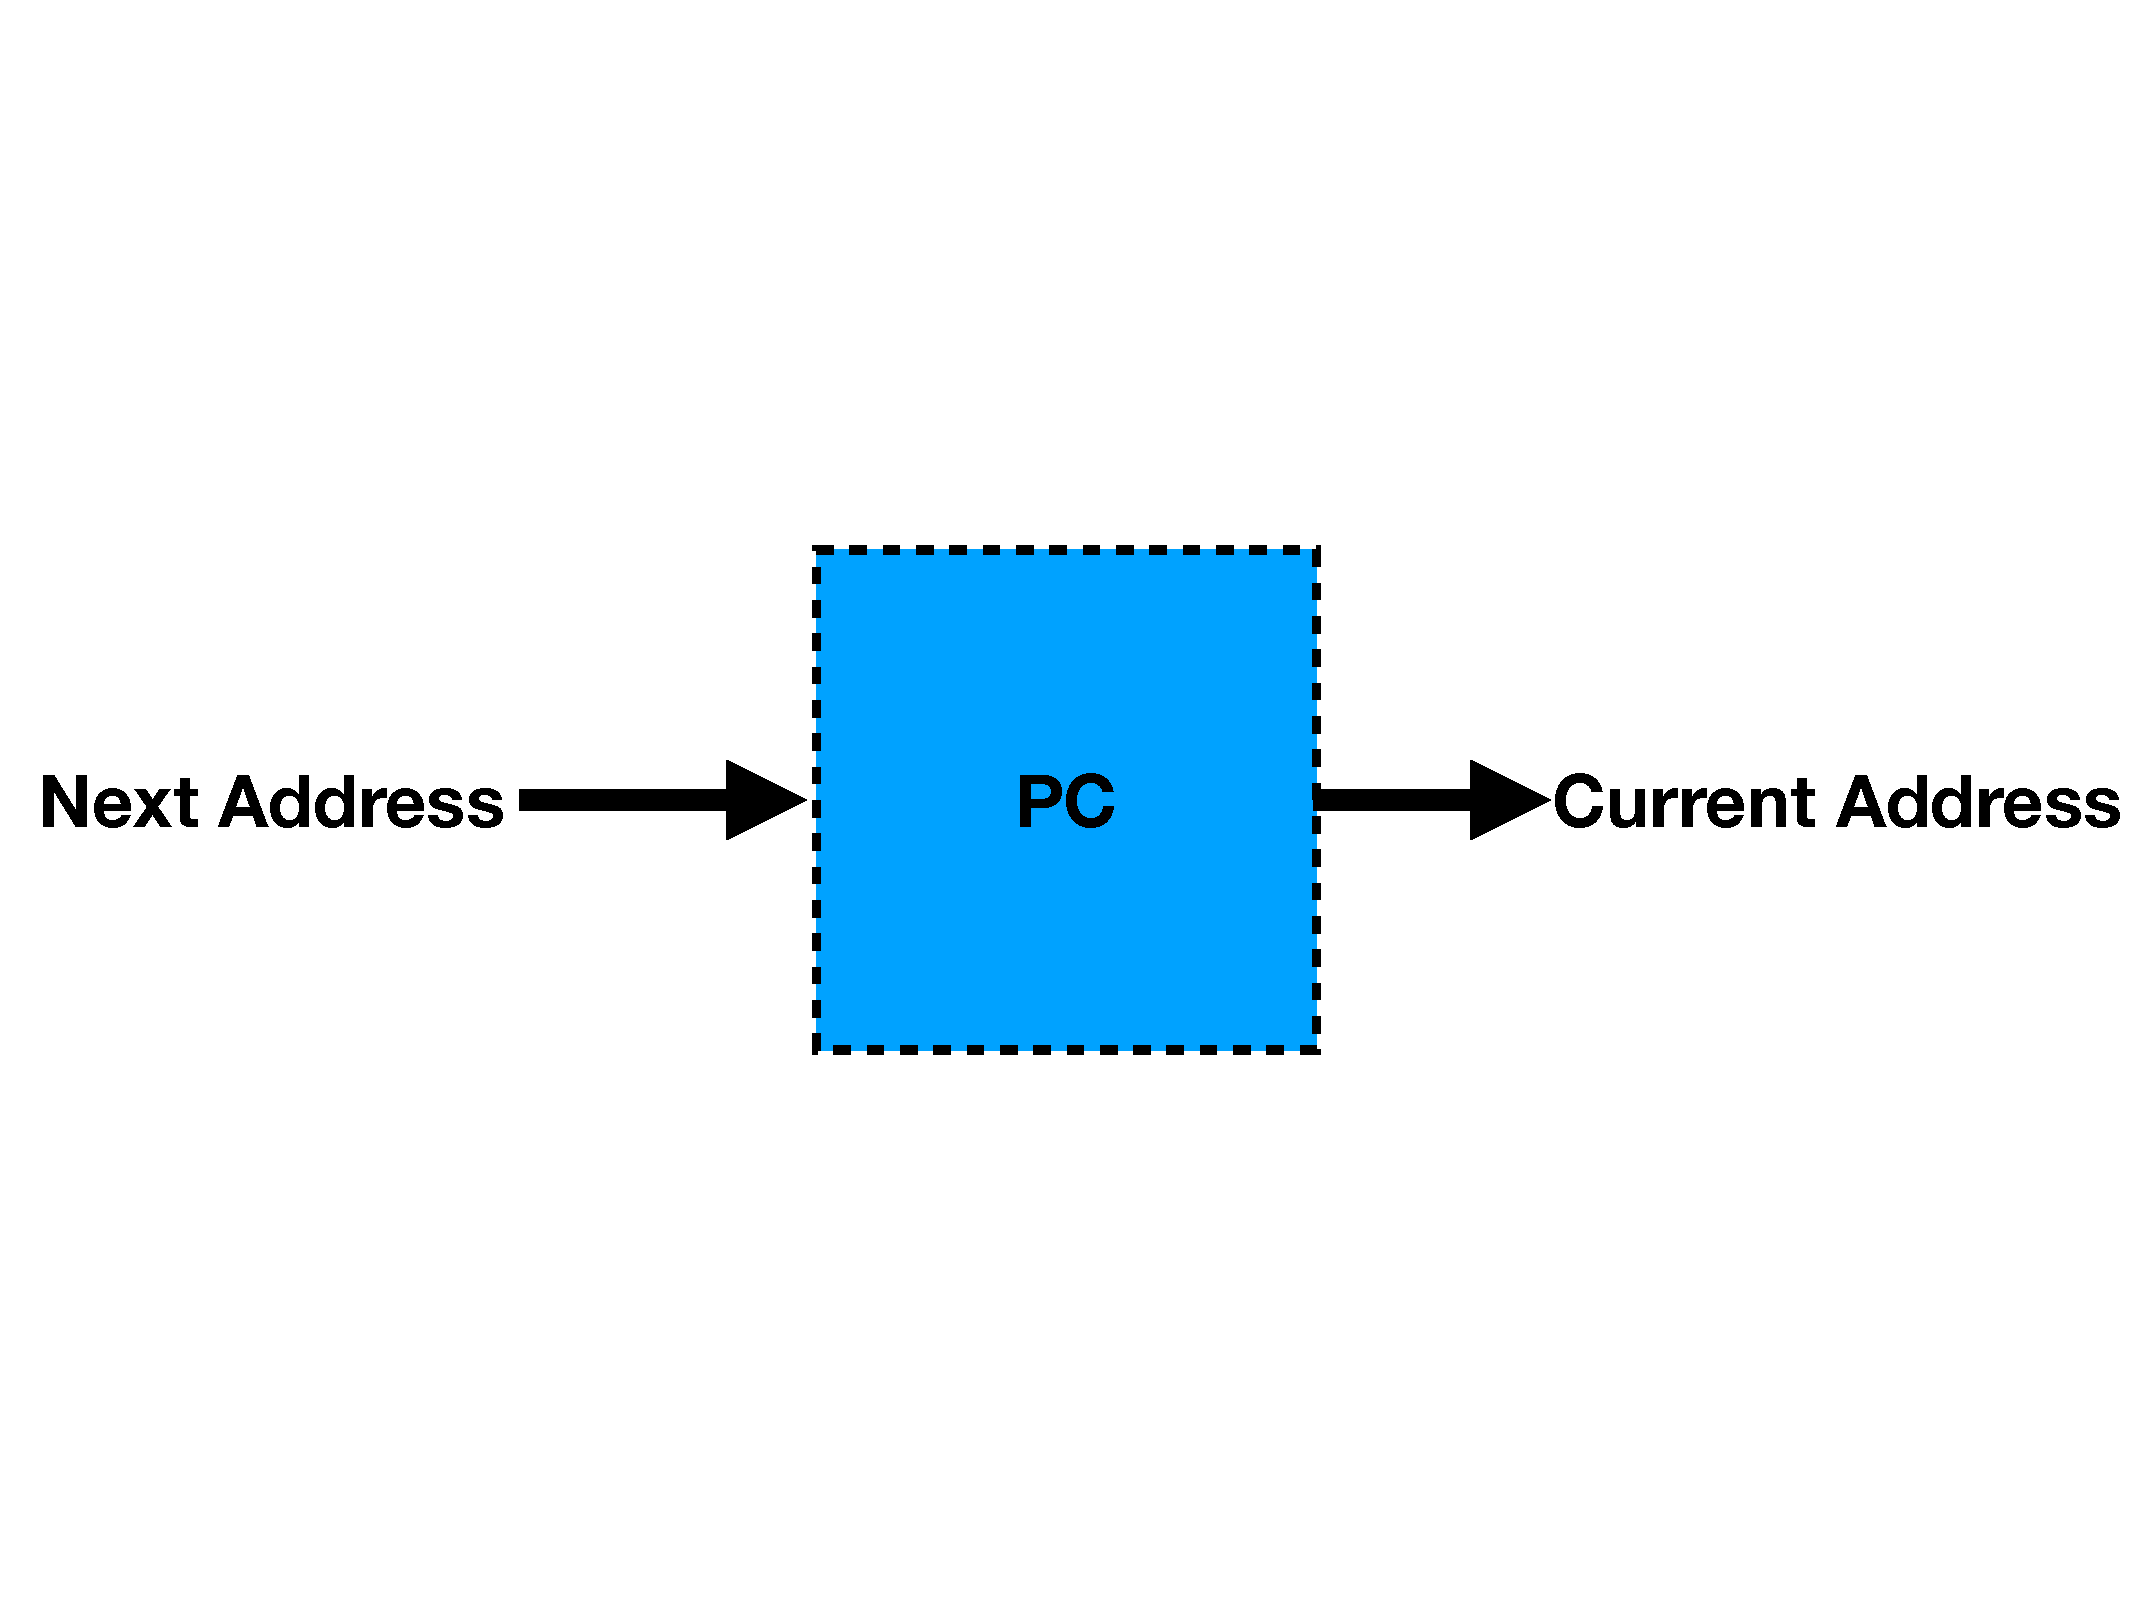
\includegraphics[scale=0.25]{pictures/PC.pdf}
            \caption{Illustration of the clocked \texttt{program counter} process having the next address as input and current address as output.}
            \label{fig:PC}
        \end{figure}
    
        \begin{minipage}{\linewidth}
            \begin{lstlisting}[language={[Sharp]C}, caption={A slice of the PC unit SME code, which contains variable that holds the input address. On every cycle edge it then holds and outputs the current address.},captionpos=b, label = PCSME]
...
    ulong address_hold;

    protected override void OnTick() {
        address_hold = m_Input.Address;
        Output.Address = address_hold;
    }
            \end{lstlisting}
        \end{minipage}   
    
    \subsection{Instruction Memory}
        The \textit{instruction memory}, IM for short, contains the program to be run on the CPU. To implement the instruction memory we create a SME process. It contains a byte array with the instructions to be run. A byte array was chosen to respect the conventions discussed in \ref{section:datatranserinstructions}. This also has the added benefit of having a built-in C$\scalerel*{\#}{X}$ function to read a binary file, which automatically puts the instructions contained within the file, in the correct array format. 
        
        The instructions can also be hand written when declaring the array. Since an instruction is 32-bits, 4 elements in the array are needed to form an instruction, where index 0-3 contains the first instruction.
        
        The instruction memory process has a single input from the program counter, which it uses access the correct instructions. In each cycle we first check whether the address given lies within the instruction array range, if not we shut down the CPU.
        We then construct an instruction, using methods discussed in \ref{section:Operators}, to a temporary variable.
        
        The register fields are then sliced out of this variable and put in the corresponding output buses, \texttt{Read RS1, RS2} and \texttt{Write RS}. The full instruction is also outputted to its own bus, \texttt{instruction}. Lastly we tell the simulation process to keep the CPU running by asserting the \texttt{CPU} bus. The instruction memory process has been illustrated in Figure \ref{fig:IM} and a code segment is shown Listing \ref{IMSME} explaining parts of the code. 
     
        \begin{figure}[h!]
            \centering
            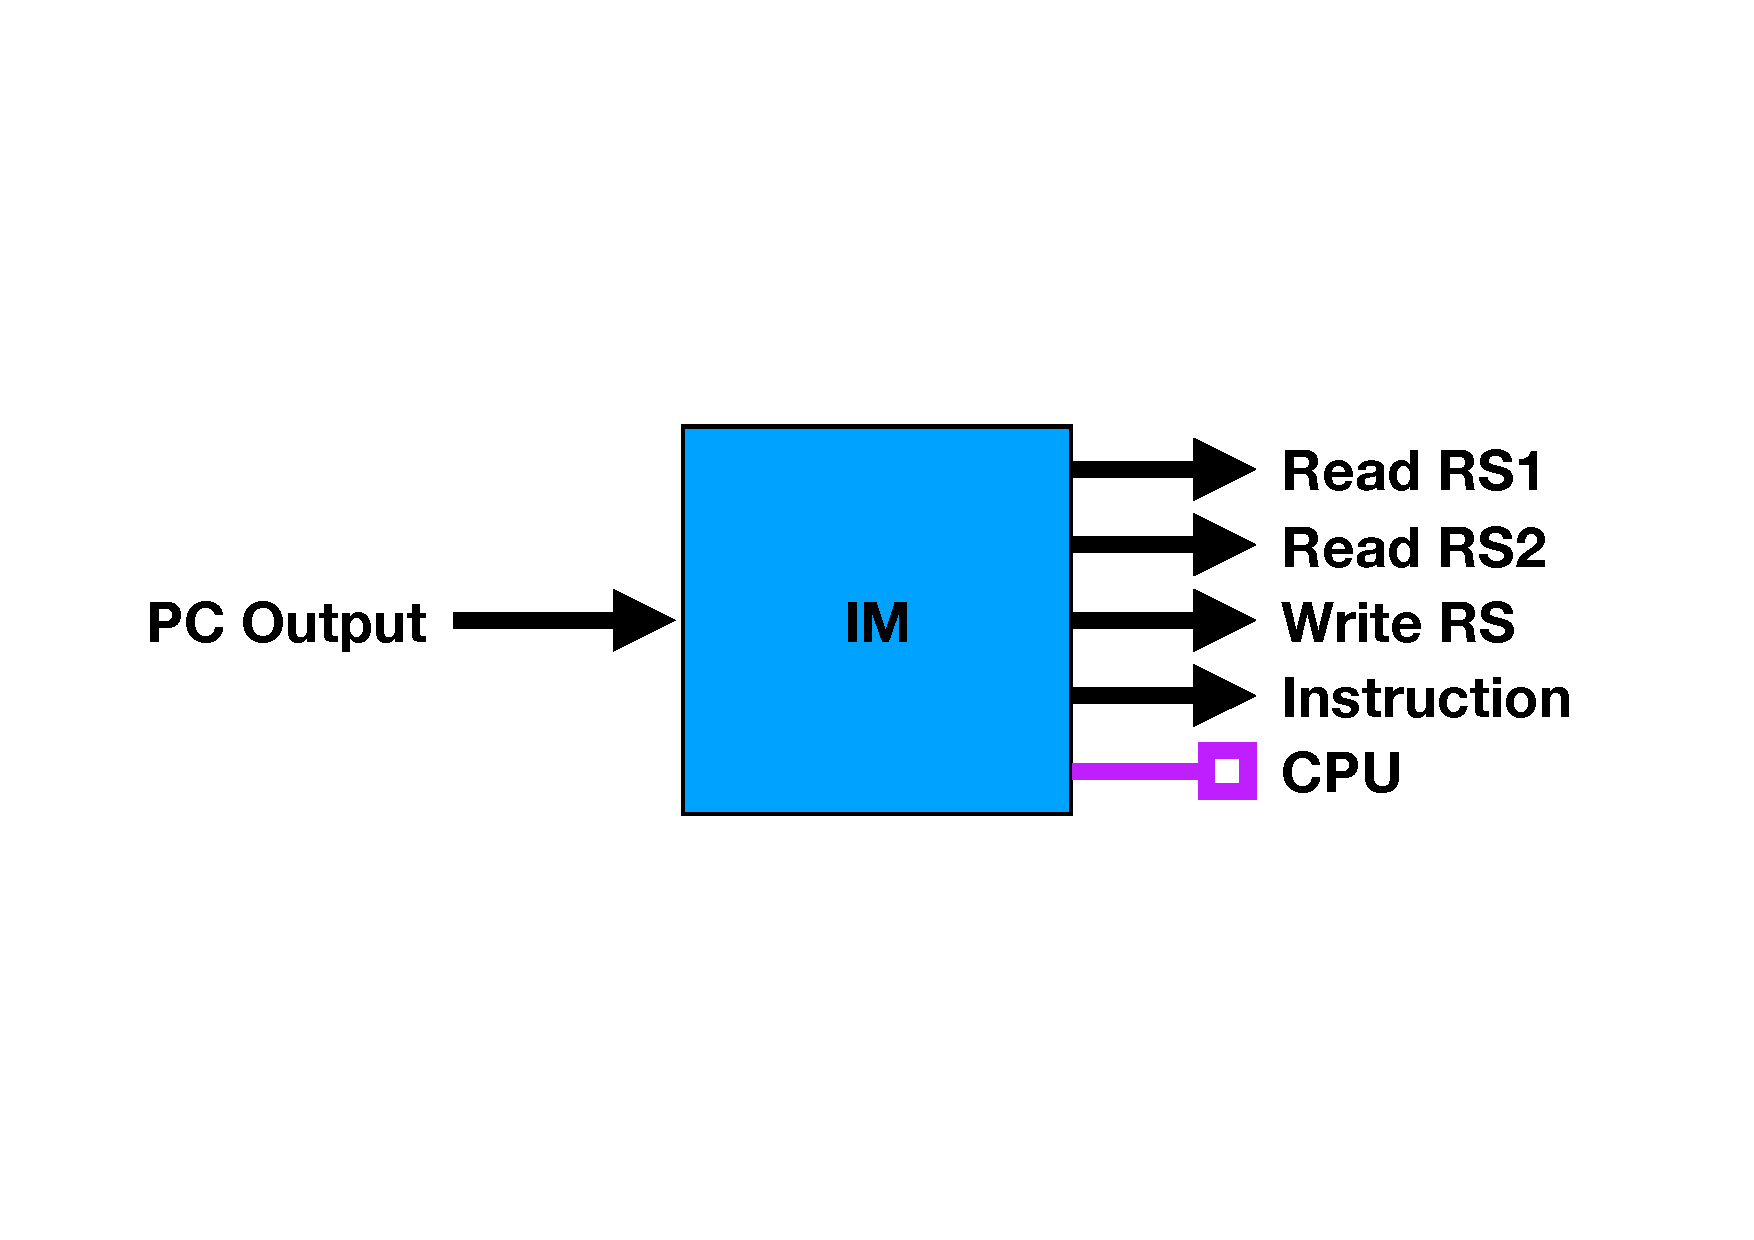
\includegraphics[scale=0.34]{pictures/IM.pdf}
            \caption{Illustration of the \texttt{instruction memory} process, taking the PC output as input and outputting to the 5 buses, \texttt{Read RS1 and RS2}, \texttt{Write RS}, \texttt{Instruction} and \texttt{CPU}.}
            \label{fig:IM}
        \end{figure}
    
        \begin{minipage}{\linewidth}
            \begin{lstlisting}[language={[Sharp]C}, caption={A slice of the Instruction Memory unit SME code. It contains a single byte array, which holds all the instructions to be run. First we check whether the given address to be accessed lies within instruction array, if not we shut down the CPU. We then use the address to access the correct array elements to create a temporary variable, which contains the instruction, as shown in lines 9-12. Hereafter we slice out the fields in the instruction and place the values in the correct busses. Lastly we tell the simulator to keep the CPU running using the CPU bus.},captionpos=b, label = IMSME]
...
    private readonly byte[] Instruction_Memory = System.IO.File.ReadAllBytes("/Users/danielramyar/Downloads/fibo.bin");
            
    protected override void OnTick() {
        ulong temp_address = m_input.Address;
        uint temp_instruction;
            
        if (temp_address >= 0 && temp_address < (uint)Instruction_Memory.Length) {
            temp_instruction = 0u | (uint)Instruction_Memory[temp_address]     << 24
                                  | (uint)Instruction_Memory[temp_address + 1] << 16
                                  | (uint)Instruction_Memory[temp_address + 2] << 8
                                  | (uint)Instruction_Memory[temp_address + 3];
            
            m_Instruction.Current = temp_instruction;
            m_read_1.Address = (uint)temp_instruction >> 15 & (uint)31; 
            m_read_2.Address = (uint)temp_instruction >> 20 & (uint)31; 
            m_write.Address  = (uint)temp_instruction >> 7  & (uint)31; 
            
            m_CPU.Running = true; // Keep CPU running
        }
        else {
            temp_instruction = 0u; // No Instruction
            ...  // Same as in the if statement
            m_CPU.Running = false; // Turn of cpu no more instructions
    }
            \end{lstlisting}
        \end{minipage}  
        
        
        
    
    \subsection{Next instruction Unit}
        To calculate the address of the next instruction in the queue I have created a unit called \texttt{Next}. This unit is very simple, as its only function is to increment the value found in the PC output bus by 4. We increment by 4, since each instruction is 32 bits long and since our instructions are contained in a byte array, we need to move 4 bytes every time we want to access the following instruction. For example if we are placed at index 0, we would have to go to index 4 to access the next instruction (index 0-3 contains instruction 1 and index 4-7 the next).
        
        The next instruction process has the the output from the program counter as input and sends the incremented address to the \texttt{Next Output} bus. The \texttt{Next} process is illustrated in \ref{fig:NEXT} and a code segment is shown in Listing \ref{NEXTSME}.
        
        \begin{figure}[h!]
            \centering
            \includegraphics[scale=0.34]{pictures/Next.pdf}
            \caption{Illustration of the \texttt{next} process, taking the \texttt{PC output} as input and outputs the next instruction adress to the \texttt{next output} bus.}
            \label{fig:NEXT}
        \end{figure}
    
        \begin{minipage}{\linewidth}
            \begin{lstlisting}[language={[Sharp]C}, caption={A slice of the \texttt{Next} process SME code. Here we declare a temporary varible, which contains the program counter output. We increment the temporary variable by four and place it in the output bus.},captionpos=b, label = NEXTSME]
...
        ulong temp;
        
        protected override void OnTick() {
            temp = m_Input.Address + 4;
            Output.Address = temp;
        }
            \end{lstlisting}
        \end{minipage}  
        
    
    \subsection{Register}
    
    \subsection{Arithmetic Logic Unit (ALU)}
    
    \subsection{Immediate generator}
    
    \subsection{Data Memory}
    \improvement{Need to figure out more sections to explain whole datapath}
    
\section{Designing the Control}
    
\section{Single Cycle RISC-V datapath}

\section{Improving the datapath} \improvement{figure out better naming for sections}

    \subsection{RV64I Base Instructions Support}

    \subsection{Supporting R-Format}
    
    \subsection{Supporting I-Format}
    
    \subsection{Supporting S-Format}
    
    \subsection{Supporting B-Format}
    
    \subsection{Supporting U-Format}
    
    \subsection{Supporting J-Format}
    
\section{Debugging the instructions}

    \subsection{Writing assembly to test instructions}
    
    \subsection{Writing simple C code to run on RISC-V}
    
    
    

    
        \chapter{Conclusion and future work}

\note{Pipeline the processor, Add necessary elements to run linux on it, add an fft instruction}



        \appendix

\chapter{Unary Operators}
\label{appendix:Unary_Operators}

    
    
    \subsubsection{Logical identity}
        
        Hereafter we have the logical identity operator which we will represent as the function $I(x)$. The logical identity operator takes an argument and returns it as is. 
        
        A logic table for the identity operator has been created and can be found in table \ref{LogicTable:Identity}. In the first column we find our preposition $p$ and its arguments. In the second column we find the return values of the identity operator with the prepositions as the argument $I(p)$.
        
        \begin{table}[h!]
            \centering
            \begin{tabular}{|c|c|}
            	\hline
            	  $p$   & $I(p)$  \\ \hline
            	$true$  & $true$  \\ \hline
            	$false$ & $false$ \\ \hline
            \end{tabular}
            \caption{Logic table of the identity operator where the proposition p, which is either true or false, can be found in the first column. In the second column we find $I(p)$, which is the identity operator with $p$ as its argument, and its return values.}
            \label{LogicTable:Identity}
        \end{table}
        
    \subsubsection{Logical true}
        
        Next we have logical true which we will represent as the function $T(x)$. Logical true takes an argument and always returns true.
        
        A logic table for the true operator has been created and can be found in table \ref{LogicTable:True}. In the first column we find our preposition $p$ and its arguments. In the second column we find the return values of the true operator with the prepositions as the argument $T(p)$.
        
        \begin{table}[h!]
            \centering
            \begin{tabular}{|c|c|}
            	\hline
            	  $p$   & $T(p)$ \\ \hline
            	$true$  & $true$ \\ \hline
            	$false$ & $true$ \\ \hline
            \end{tabular}
            \caption{Logic table of the true operator where the proposition p, which is either true or false, can be found in the first column. In the second column we find $T(p)$, which is the true operator with $p$ as its argument, and its return values.}
            \label{LogicTable:True}
        \end{table}
    
    \subsubsection{Logical false}
        
        Lastly we have logical false which we will represent as the function $F(x)$. Logical false takes an argument and always return false.
        
        A logic table for the false operator has been created and can be found in table \ref{LogicTable:False}. In the first column we find our preposition $p$ and its arguments. In the second column we find the return values of the false operator with the prepositions as the argument $F(p)$.
        
        \begin{table}[h!]
            \centering
            \begin{tabular}{|c|c|}
            	\hline
            	  $p$   & $F(p)$  \\ \hline
            	$true$  & $false$ \\ \hline
            	$false$ & $false$ \\ \hline
            \end{tabular}
            \caption{Logic table of the false operator where the proposition p, which is either true or false, can be found in the first column. In the second column we find $F(p)$, which is the false operator with $p$ as its argument, and its return values.}
            \label{LogicTable:False}
    \end{table}

\chapter{Binary Operators}
\label{appendix:Binaray_Operators}
    \subsubsection{Joint denial}
        Joint denial is represented by $\downarrow$ in mathematics or NOR in computer science and commonly referred to as the NOR operator. The NOR operator results in a true value only if both operands are false.
        
        Using table \ref{LogicTable:PossibleOperators} we see that the set of outputs which corresponds to this definition is column 15 and is summarized in table \ref{LogicTable:NOR}.
        
        Here we have the propositions $p$ and $q$ in the first two columns and all possible permutations between them in the following rows. The last column then shows the resulting value after doing the NOR operation between $p$ and $q$.
        
        \begin{table}[h!]
            \centering
            \begin{tabular}{|c|c|c|}
            	\hline
            	  $p$   &   $q$   & $p \downarrow q$ \\ \hline
            	$true$  & $true$  &     $false$      \\ \hline
            	$true$  & $false$ &     $false$      \\ \hline
            	$false$ & $true$  &     $false$      \\ \hline
            	$false$ & $false$ &      $true$      \\ \hline
            \end{tabular}
            \caption{Logic table of the NOR operator where $p$ is the first proposition and $q$ is the second. All possible permutations are then specified in each row for each proposition. The third column then shows the resulting value of the NOR operation between $p$ and $q$.}
            \label{LogicTable:NOR}
        \end{table}
        
        In disjunctive normal form the NOR operator can be expressed in the following form
        \begin{equation}
            p \downarrow q = (\neg p \wedge \neg q)
        \end{equation}
        using the procedure mentioned in chapter \ref{section:Boolean_algebra}.
    
    \subsubsection{Alternative denial}
        Alternative denial is represented by $\uparrow$ in mathematics or NAND in computer science and commonly referred to as the NAND operator. The NAND operator results in a true value only if one or more of the operands are false.
        
        Using table \ref{LogicTable:PossibleOperators} we see that the set of outputs which corresponds to this definition is column 5 and is summarized in table \ref{LogicTable:NAND}.
        
        Here we have the propositions $p$ and $q$ in the first two columns and all possible permutations between them in the following rows. The last column then shows the resulting value after doing the NAND operation between $p$ and $q$.
        
        \begin{table}[h!]
            \centering
            \begin{tabular}{|c|c|c|}
            	\hline
            	  $p$   &   $q$   & $p \uparrow q$ \\ \hline
            	$true$  & $true$  &    $false$     \\ \hline
            	$true$  & $false$ &     $true$     \\ \hline
            	$false$ & $true$  &     $true$     \\ \hline
            	$false$ & $false$ &     $true$     \\ \hline
            \end{tabular}
            \caption{Logic table of the NAND operator where $p$ is the first proposition and $q$ is the second. All possible permutations are then specified in each row for each proposition. The third column then shows the resulting value of the NAND operation between $p$ and $q$.}
            \label{LogicTable:NAND}
        \end{table}
        
        In disjunctive normal form the NAND operator can be expressed in the following form
        \begin{equation}
            p \uparrow q = (p \wedge \neg q) \vee (\neg p \wedge q) \vee (\neg p \wedge \neg q)
        \end{equation}
        using the procedure mentioned in chapter \ref{section:Boolean_algebra}.
    
    \subsubsection{Logical biconditional}
        The logical biconditional is represented by $\leftrightarrow$ in mathematics or XNOR in computer science and commonly referred to as the exclusive NOR operator. The XNOR operator results in a true value only if both operands are either true or false.
        
        Using table \ref{LogicTable:PossibleOperators} we see that the set of outputs which corresponds to this definition is column 9 and is summarized in table \ref{LogicTable:XNOR}.
        
        Here we have the propositions $p$ and $q$ in the first two columns and all possible permutations between them in the following rows. The last column then shows the resulting value after doing the XNOR operation between $p$ and $q$.
        
        \begin{table}[h!]
            \centering
            \begin{tabular}{|c|c|c|}
            	\hline
            	  $p$   &   $q$   & $p \leftrightarrow q$ \\ \hline
            	$true$  & $true$  &        $true$         \\ \hline
            	$true$  & $false$ &        $false$        \\ \hline
            	$false$ & $true$  &        $false$        \\ \hline
            	$false$ & $false$ &        $true$         \\ \hline
            \end{tabular}
            \caption{Logic table of the XNOR operator where $p$ is the first proposition and $q$ is the second. All possible permutations are then specified in each row for each proposition. The third column then shows the resulting value of the XNOR operation between $p$ and $q$.}
            \label{LogicTable:XNOR}
        \end{table}
        
        In disjunctive normal form the XNOR operator can be expressed in the following form
        \begin{equation}
            p \leftrightarrow q = (p \wedge  q) \vee (\neg p \wedge \neg q)
        \end{equation}
        using the procedure mentioned in chapter \ref{section:Boolean_algebra}.


    \subsubsection{Tautology}
        The tautology operator is represented by $\top$ in mathematics which always returns a true value.
        
        Using table \ref{LogicTable:PossibleOperators} we see that the set of outputs which corresponds to this definition is column 1 and is summarized in table \ref{LogicTable:tautology}.
        
        Here we have the propositions $p$ and $q$ in the first two columns and all possible permutations between them in the following rows. The last column then shows the resulting value after doing the tautology operation between $p$ and $q$.
        
        \begin{table}[h!]
            \centering
            \begin{tabular}{|c|c|c|}
            	\hline
            	  $p$   &   $q$   & $p \top q$ \\ \hline
            	$true$  & $true$  &   $true$   \\ \hline
            	$true$  & $false$ &   $true$   \\ \hline
            	$false$ & $true$  &   $true$   \\ \hline
            	$false$ & $false$ &   $true$   \\ \hline
            \end{tabular}
            \caption{Logic table of the tautology operator where $p$ is the first proposition and $q$ is the second. All possible permutations are then specified in each row for each proposition. The third column then shows the resulting value of the tautology operation between $p$ and $q$.}
            \label{LogicTable:tautology}
        \end{table}
        
        In disjunctive normal form the tautology operator can be expressed in the following form
        \begin{equation}
            p \top q = (p \wedge q) \vee (p \wedge \neg q) \vee (\neg p \wedge q) \vee (\neg p \wedge \neg q)
        \end{equation}
        using the procedure mentioned in chapter \ref{section:Boolean_algebra}.
    
    \subsubsection{Contradiction}
        The contradiction operator is represented by $\bot$ in mathematics which always returns a false value.
        
        Using table \ref{LogicTable:PossibleOperators} we see that the set of outputs which corresponds to this definition is column 16 and is summarized in table \ref{LogicTable:contradiction}.
        
        Here we have the propositions $p$ and $q$ in the first two columns and all possible permutations between them in the following rows. The last column then shows the resulting value after doing the contradiction operator between $p$ and $q$.
        
        \begin{table}[h!]
            \centering
            \begin{tabular}{|c|c|c|}
            	\hline
            	  $p$   &   $q$   & $p \bot q$ \\ \hline
            	$true$  & $true$  &  $false$   \\ \hline
            	$true$  & $false$ &  $false$   \\ \hline
            	$false$ & $true$  &  $false$   \\ \hline
            	$false$ & $false$ &  $false$   \\ \hline
            \end{tabular}
            \caption{Logic table of the contradiction operator where $p$ is the first proposition and $q$ is the second. All possible permutations are then specified in each row for each proposition. The third column then shows the resulting value of the contradiction operation between $p$ and $q$.}
            \label{LogicTable:contradiction}
        \end{table}
        
        In disjunctive normal form the contradiction operator can be expressed in the following form
        \begin{equation}
            p \bot q = p \wedge \neg p
        \end{equation}
    
    \subsubsection{Proposition P}
        We will define the operator Proposition P which results in a true value only if the first operand p is true.
        
        Using table \ref{LogicTable:PossibleOperators} we see that the set of outputs which corresponds to this definition is column 6 and is summarized in table \ref{LogicTable:P}.
        
        Here we have the propositions $p$ and $q$ in the first two columns and all possible permutations between them in the following rows. The last column then shows the resulting value after doing the proposition P between $p$ and $q$.
        
        \begin{table}[h!]
            \centering
            \begin{tabular}{|c|c|c|}
            	\hline
            	  $p$   &   $q$   & $P(p, q)$ \\ \hline
            	$true$  & $true$  &  $true$   \\ \hline
            	$true$  & $false$ &  $true$   \\ \hline
            	$false$ & $true$  &  $false$  \\ \hline
            	$false$ & $false$ &  $false$  \\ \hline
            \end{tabular}
            \caption{Logic table of the proposition P operator where $p$ is the first proposition and $q$ is the second. All possible permutations are then specified in each row for each proposition. The third column then shows the resulting value of the proposition P operation between $p$ and $q$.}
            \label{LogicTable:P}
        \end{table}
        
        In disjunctive normal form the proposition P can be expressed in the following form
        \begin{equation}
            P(p, q) = (p \wedge q) \vee (p \wedge \neg q)
        \end{equation}
        using the procedure mentioned in chapter \ref{section:Boolean_algebra}.
    
    \subsubsection{Proposition Q}
        We will define the operator Proposition Q which results in a true value only if the second operand q is true.
        
        Using table \ref{LogicTable:PossibleOperators} we see that the set of outputs which corresponds to this definition is column 10 and is summarized in table \ref{LogicTable:Q}.
        
        Here we have the propositions $p$ and $q$ in the first two columns and all possible permutations between them in the following rows. The last column then shows the resulting value after doing the proposition Q between $p$ and $q$.
        
        \begin{table}[h!]
            \centering
            \begin{tabular}{|c|c|c|}
            	\hline
            	  $p$   &   $q$   & $Q(p, q)$ \\ \hline
            	$true$  & $true$  &  $true$   \\ \hline
            	$true$  & $false$ &  $false$  \\ \hline
            	$false$ & $true$  &  $true$   \\ \hline
            	$false$ & $false$ &  $false$  \\ \hline
            \end{tabular}
            \caption{Logic table of the proposition P operator where $p$ is the first proposition and $q$ is the second. All possible permutations are then specified in each row for each proposition. The third column then shows the resulting value of the proposition P operation between $p$ and $q$.}
            \label{LogicTable:Q}
        \end{table}
        
        In disjunctive normal form the proposition Q can be expressed in the following form
        \begin{equation}
            P(p, q) = (p \wedge q) \vee (\neg p \wedge  q)
        \end{equation}
        using the procedure mentioned in chapter \ref{section:Boolean_algebra}.
    
    \subsubsection{Negated P}
        We will define the operator negated P which results in a true value only if the first operand p is false.
        
        Using table \ref{LogicTable:PossibleOperators} we see that the set of outputs which corresponds to this definition is column 8 and is summarized in table \ref{LogicTable:NOTP}.
        
        Here we have the propositions $p$ and $q$ in the first two columns and all possible permutations between them in the following rows. The last column then shows the resulting value after doing the negated P between $p$ and $q$.
        
        \begin{table}[h!]
            \centering
            \begin{tabular}{|c|c|c|}
            	\hline
            	  $p$   &   $q$   & $\neg P(p, q)$ \\ \hline
            	$true$  & $true$  &    $false$     \\ \hline
            	$true$  & $false$ &    $false$     \\ \hline
            	$false$ & $true$  &     $true$     \\ \hline
            	$false$ & $false$ &     $true$     \\ \hline
            \end{tabular}
            \caption{Logic table of the negated P operator where $p$ is the first proposition and $q$ is the second. All possible permutations are then specified in each row for each proposition. The third column then shows the resulting value of the negated P operation between $p$ and $q$.}
            \label{LogicTable:NOTP}
        \end{table}
        
        In disjunctive normal form the negated P can be expressed in the following form
        \begin{equation}
            \neg P(p, q) = (\neg p \wedge  q) \vee (\neg p \wedge \neg q)
        \end{equation}
        using the procedure mentioned in chapter \ref{section:Boolean_algebra}.
        
    \subsubsection{Negated Q}
        We will define the operator negated Q which results in a true value only if the second operand q is false.
        
        Using table \ref{LogicTable:PossibleOperators} we see that the set of outputs which corresponds to this definition is column 11 and is summarized in table \ref{LogicTable:NOTQ}.
        
        Here we have the propositions $p$ and $q$ in the first two columns and all possible permutations between them in the following rows. The last column then shows the resulting value after doing the negated Q between $p$ and $q$.
        
        \begin{table}[h!]
            \centering
            \begin{tabular}{|c|c|c|}
            	\hline
            	  $p$   &   $q$   & $\neg Q(p, q)$ \\ \hline
            	$true$  & $true$  &    $false$     \\ \hline
            	$true$  & $false$ &     $true$     \\ \hline
            	$false$ & $true$  &    $false$     \\ \hline
            	$false$ & $false$ &     $true$     \\ \hline
            \end{tabular}
            \caption{Logic table of the negated Q operator where $p$ is the first proposition and $q$ is the second. All possible permutations are then specified in each row for each proposition. The third column then shows the resulting value of the negated operation between $p$ and $q$.}
            \label{LogicTable:NOTQ}
        \end{table}
        
        In disjunctive normal form the negated Q can be expressed in the following form
        \begin{equation}
            \neg Q(p, q) = (p \wedge \neg q) \vee (\neg p \wedge \neg q)
        \end{equation}
        using the procedure mentioned in chapter \ref{section:Boolean_algebra}.
        
    \subsubsection{Material implication}
        Material implication is represented by $\rightarrow$ in mathematics. The material implication operator results in a false value only if the first operand p is true and second operand q is false.
        
        Using table \ref{LogicTable:PossibleOperators} we see that the set of outputs which corresponds to this definition is column 4 and is summarized in table \ref{LogicTable:MI}.
        
        Here we have the propositions $p$ and $q$ in the first two columns and all possible permutations between them in the following rows. The last column then shows the resulting value after doing the material implication operation between $p$ and $q$.
        
        \begin{table}[h!]
            \centering
            \begin{tabular}{|c|c|c|}
            	\hline
            	  $p$   &   $q$   & $p \rightarrow q$ \\ \hline
            	$true$  & $true$  &      $true$       \\ \hline
            	$true$  & $false$ &      $false$      \\ \hline
            	$false$ & $true$  &      $true$       \\ \hline
            	$false$ & $false$ &      $true$       \\ \hline
            \end{tabular}
            \caption{Logic table of the material implication operator where $p$ is the first proposition and $q$ is the second. All possible permutations are then specified in each row for each proposition. The third column then shows the resulting value of the material implication operation between $p$ and $q$.}
            \label{LogicTable:MI}
        \end{table}
        
        In disjunctive normal form the material implication operator can be expressed in the following form
        \begin{equation}
            p \rightarrow q = (p \wedge  q) \vee (\neg p \wedge q) \vee (\neg p \wedge \neg q)
        \end{equation}
        using the procedure mentioned in chapter \ref{section:Boolean_algebra}.
    
    
    \subsubsection{Converse implication}
        Converse implication is represented by $\leftarrow$ in mathematics. The converse implication operator results in a false value only if the first operand p is true and the second q is true.
        
        Using table \ref{LogicTable:PossibleOperators} we see that the set of outputs which corresponds to this definition is column 3 and is summarized in table \ref{LogicTable:CI}.
        
        Here we have the propositions $p$ and $q$ in the first two columns and all possible permutations between them in the following rows. The last column then shows the resulting value after doing the converse implication operation between $p$ and $q$.
        
        \begin{table}[h!]
            \centering
            \begin{tabular}{|c|c|c|}
            	\hline
            	  $p$   &   $q$   & $p \leftarrow q$ \\ \hline
            	$true$  & $true$  &      $true$      \\ \hline
            	$true$  & $false$ &      $true$      \\ \hline
            	$false$ & $true$  &     $false$      \\ \hline
            	$false$ & $false$ &      $true$      \\ \hline
            \end{tabular}
            \caption{Logic table of the converse implication operator where $p$ is the first proposition and $q$ is the second. All possible permutations are then specified in each row for each proposition. The third column then shows the resulting value of the converse implication operation between $p$ and $q$.}
            \label{LogicTable:CI}
        \end{table}
        
        In disjunctive normal form the converse implication operator can be expressed in the following form
        \begin{equation}
            p \leftarrow q = (p \wedge  q) \vee (p \wedge \neg q) \vee (\neg p \wedge \neg q)
        \end{equation}
        using the procedure mentioned in chapter \ref{section:Boolean_algebra}.
    
    \subsubsection{Material nonimplication}
        Material nonimplication is represented by $\not\rightarrow$ in mathematics. The material nonimplication operator results in a true value only if the first operand p is true and the second operand q is false.
        
        Using table \ref{LogicTable:PossibleOperators} we see that the set of outputs which corresponds to this definition is column 13 and is summarized in table \ref{LogicTable:MNI}.
        
        Here we have the propositions $p$ and $q$ in the first two columns and all possible permutations between them in the following rows. The last column then shows the resulting value after doing the material nonimplication operation between $p$ and $q$.
        
        \begin{table}[h!]
            \centering
            \begin{tabular}{|c|c|c|}
            	\hline
            	  $p$   &   $q$   & $p \not\rightarrow q$ \\ \hline
            	$true$  & $true$  &        $false$        \\ \hline
            	$true$  & $false$ &        $true$         \\ \hline
            	$false$ & $true$  &        $false$        \\ \hline
            	$false$ & $false$ &        $false$        \\ \hline
            \end{tabular}
            \caption{Logic table of the material nonimplication operator where $p$ is the first proposition and $q$ is the second. All possible permutations are then specified in each row for each proposition. The third column then shows the resulting value of the material nonimplication operation between $p$ and $q$.}
            \label{LogicTable:MNI}
        \end{table}
        
        In disjunctive normal form the material nonimplication operator can be expressed in the following form
        \begin{equation}
            p \rightarrow q = p \wedge \neg q 
        \end{equation}
        using the procedure mentioned in chapter \ref{section:Boolean_algebra}.
    
    \subsubsection{Converse nonimplication}
        Converse nonimplication is represented by $\not\leftarrow$ in mathematics. The converse nonimplication operator results in a true value only if the first operand p is false and the second operand q is true.
        
        Using table \ref{LogicTable:PossibleOperators} we see that the set of outputs which corresponds to this definition is column 14 and is summarized in table \ref{LogicTable:CNI}.
        
        Here we have the propositions $p$ and $q$ in the first two columns and all possible permutations between them in the following rows. The last column then shows the resulting value after doing the converse nonimplication operation between $p$ and $q$.
        
        \begin{table}[h!]
            \centering
            \begin{tabular}{|c|c|c|}
            	\hline
            	  $p$   &   $q$   & $p \not\leftarrow q$ \\ \hline
            	$true$  & $true$  &       $false$        \\ \hline
            	$true$  & $false$ &       $false$        \\ \hline
            	$false$ & $true$  &        $true$        \\ \hline
            	$false$ & $false$ &       $false$        \\ \hline
            \end{tabular}
            \caption{Logic table of the converse nonimplication operator where $p$ is the first proposition and $q$ is the second. All possible permutations are then specified in each row for each proposition. The third column then shows the resulting value of the converse nonimplication operation between $p$ and $q$.}
            \label{LogicTable:CNI}
        \end{table}
        
        In disjunctive normal form the converse nonimplication operator can be expressed in the following form
        \begin{equation}
            p \leftarrow q =\neg p \wedge q
        \end{equation}
        using the procedure mentioned in chapter \ref{section:Boolean_algebra}.
    \end{onehalfspacing}

    \vspace*{-2cm}
\section*{Risc V Reference Card}

\subsection*{Instruction Formats}
    \begin{table}[h]
        \scriptsize
        \begin{tabular} %In the table specs i create 32 even size colums and 1 coloum for text
            {p{0.01mm}p{0.01mm}p{0.01mm}p{0.01mm} p{0.01mm}p{0.01mm}p{0.01mm}p{0.01mm}
             p{0.01mm}p{0.01mm}p{0.01mm}p{0.01mm} p{0.01mm}p{0.01mm}p{0.01mm}p{0.01mm}
             p{0.01mm}p{0.01mm}p{0.01mm}p{0.01mm} p{0.01mm}p{0.01mm}p{0.01mm}p{0.01mm}
             p{0.01mm}p{0.01mm}p{0.01mm}p{0.01mm} p{0.01mm}p{0.01mm}p{0.01mm}p{0.01mm} l}
            %Here we create the row for the bit numbers (only relevant ones are filled for space)
            \multicolumn{1}{c}{31}&&&&&&
            \multicolumn{1}{c}{25}&
            \multicolumn{1}{c}{24}&&&&
            \multicolumn{1}{c}{20}&
            \multicolumn{1}{c}{19}&&&&
            \multicolumn{1}{c}{15}&
            \multicolumn{1}{c}{14}&&&
            \multicolumn{1}{c}{11}&&&&
            \multicolumn{1}{c}{7}&
            \multicolumn{1}{c}{6}&&&&&&
            \multicolumn{1}{c}{0}&
            \\
            %Here we create the R-type row
            \cline{0-31} 
            \multicolumn{7}{|c|}{funct7} &
            \multicolumn{5}{c|}{rs2}&
            \multicolumn{5}{c|}{rs1}&
            \multicolumn{3}{c|}{funct3}&
            \multicolumn{5}{c|}{rd}&
            \multicolumn{7}{c|}{opcode}&
            R-type
            \\
            %Here we create the I-type row
            \cline{0-31} 
            \multicolumn{12}{|c|}{imm[11:0]} &
            \multicolumn{5}{c|}{rs1}&
            \multicolumn{3}{c|}{funct3}&
            \multicolumn{5}{c|}{rd}&
            \multicolumn{7}{c|}{opcode}&
            I-type
            \\
            %Here we create the special case I-type row
            \cline{0-31} 
            \multicolumn{6}{|c|}{imm[11:5]} &
            \multicolumn{1}{|c|}{imm[5]} &
            \multicolumn{5}{c|}{imm[4:0]}&
            \multicolumn{5}{c|}{rs1}&
            \multicolumn{3}{c|}{funct3}&
            \multicolumn{5}{c|}{rd}&
            \multicolumn{7}{c|}{opcode}&
            I-type\textsuperscript{*}
            \\
            %Here we create the S-type row
            \cline{0-31} 
            \multicolumn{7}{|c|}{imm[11:5]} &
            \multicolumn{5}{c|}{rs2}&
            \multicolumn{5}{c|}{rs1}&
            \multicolumn{3}{c|}{imm[4:0]}&
            \multicolumn{5}{c|}{rd}&
            \multicolumn{7}{c|}{opcode}&
            S-type
            \\
            %Here we create the B-type row
            \cline{0-31} 
            \multicolumn{7}{|c|}{imm[12$|$10:5]} &
            \multicolumn{5}{c|}{rs2}&
            \multicolumn{5}{c|}{rs1}&
            \multicolumn{3}{c|}{imm[4:1$|$11]}&
            \multicolumn{5}{c|}{rd}&
            \multicolumn{7}{c|}{opcode}&
            B-type
            \\
            %Here we create the U-type row
            \cline{0-31} 
            \multicolumn{20}{|c|}{imm[31:12]} &
            \multicolumn{5}{c|}{rd}&
            \multicolumn{7}{c|}{opcode}&
            U-type
            \\
            %Here we create the J-type row
            \cline{0-31} 
            \multicolumn{20}{|c|}{imm[20$|$10:1$|$11$|$19:12]} &
            \multicolumn{5}{c|}{rd}&
            \multicolumn{7}{c|}{opcode}&
            J-type
            \\
            \cline{0-31} 
        \end{tabular}
        \caption*{\small\textsuperscript{*} This is a special case of the RV64I I-type format used by slli, srli and srai instructions where the lower 6 bits (imm[5] and imm[4:0]) are used to determine the shift amount (shamt). If slliw, srliw and sraiw are used it should generate an error if imm[5] $\neq 0$}
    \end{table}
\vspace*{-0.5cm}
\subsection*{RV64I Base Instructions}
    \newcommand{\funct}{\vtop{\hbox{\strut Funct7/}\hbox{\strut imm[11:5]}}}
    \newcommand{\qast}{\textsuperscript{*}}
    \newcommand{\qdag}{\textsuperscript{$\dagger$}}
    \begin{table}[h!]
        \scriptsize
        \begin{tabular}{|l|l|l|c|l|l|l|}
        	\hline
        	Name                                  & Fmt & Opcode  & Funct3 & \funct  & Assembly            & Description (in C)             \\
            \hline
        	Add                                   & R   & 0110011 &  000   & 0000000 & add rd, rs1, rs2    & rd = rs1 $+$ rs2               \\
        	Subtract                              & R   & 0110011 &  000   & 0100000 & sub rd, rs1, rs2    & rd = rs1 $-$ rs2               \\
        	AND                                   & R   & 0110011 &  111   & 0000000 & and rd, rs1, rs2    & rd = rs1 \& rs2                \\
        	OR                                    & R   & 0110011 &  110   & 0000000 & or rd, rs1, rs2     & rd = rs1 $|$ rs2               \\
        	XOR                                   & R   & 0110011 &  100   & 0000000 & xor rd, rs1, rs2    & rd = rs1 \^{} rs2              \\
        	Shift Left Logical                    & R   & 0110011 &  001   & 0000000 & sll rd, rs1, rs2    & rd = rs1 $\ll$ rs2             \\
        	Set Less Than                         & R   & 0110011 &  010   & 0000000 & slt rd, rs1, rs2    & rd = (rs1 $<$ rs2)?1:0         \\
        	Set Less Than (U)\qast                & R   & 0110011 &  011   & 0000000 & sltu rd, rs1, rs2   & rd = (rs1 $<$ rs2)?1:0         \\
        	Shift Right Logical                   & R   & 0110011 &  101   & 0000000 & srl rd, rs1, rs2    & rd = rs1 $\gg$ rs2             \\
        	Shift Right Arithmetic\qdag           & R   & 0110011 &  101   & 0100000 & sra rd, rs1, rs2    & rd = rs1 $\gg$ rs2             \\
            \hline
            Add Word                              & R   & 0111011 &  000   & 0000000 & addw rd, rs1, rs2   & rd = rs1 $+$ rs2               \\
            Subtract Word                         & R   & 0111011 &  000   & 0100000 & subw rd, rs1, rs2   & rd = rs1 $-$ rs2               \\
            Shift Left Logical Word               & R   & 0111011 &  001   & 0000000 & sllw rd, rs1, rs2   & rd = rs1 $\ll$ rs2             \\
            Shift Right Logical Word              & R   & 0111011 &  101   & 0000000 & srlw rd, rs1, rs2   & rd = rs1 $\gg$ rs2             \\
            Shift Right Arithmetic Word\qdag      & R   & 0111011 &  101   & 0100000 & sraw rd, rs1, rs2   & rd = rs1 $\gg$ rs2             \\
            \hline
        	Add Immediate                         & I   & 0010011 &  000   &         & addi rd, rs1, imm   & rd = rs1 $+$ imm               \\
        	AND Immediate                         & I   & 0010011 &  111   &         & and rd, rs1, imm    & rd = rs1 \& imm                \\
        	OR Immediate                          & I   & 0010011 &  110   &         & or rd, rs1, imm     & rd = rs1 $|$ imm               \\
        	XOR Immediate                         & I   & 0010011 &  100   &         & xor rd, rs1, imm    & rd = rs1 \^{} imm              \\
        	Shift Left Logical Immediate          & I   & 0010011 &  001   & 0000000 & slli rd, rs1, shamt & rd = rs1 $\ll$ shamt           \\
        	Shift Right Logical Immediate         & I   & 0010011 &  101   & 0000000 & srli rd, rs1, shamt & rd = rs1 $\gg$ shamt           \\
        	Shift Right Arithmetic Immediate\qdag & I   & 0010011 &  101   & 0100000 & srai rd, rs1, shamt & rd = rs1 $\gg$ shamt           \\
        	Set Less Than Immediate               & I   & 0010011 &  010   &         & slti rd, rs1, imm   & rd = (rs1 $<$ imm)?1:0         \\
        	Set Less Than Immediate (U)\qast      & I   & 0010011 &  011   &         & sltiu rd, rs1, imm  & rd = (rs1 $<$ imm)?1:0         \\
            \hline
            Add Immediate Word                    & I   & 0011011 &  000   &         & addiw rd, rs1, imm  & rd = rs1 $+$ imm               \\
            Shift Left Logical Immediate Word     & I   & 0011011 &  001   & 0000000 & slliw rd, rs1, shamt& rd = rs1 $\ll$ shamt           \\
            Shift Right Logical Immediate Word    & I   & 0011011 &  101   & 0000000 & srliw rd, rs1, shamt& rd = rs1 $\gg$ shamt           \\
            Shift Right Arithmetic Imm Word\qdag  & I   & 0011011 &  101   & 0100000 & sraiw rd, rs1, shamt& rd = rs1 $\gg$ shamt           \\
            \hline
        	Load Byte                             & I   & 0000011 &  000   &         & lb rd, rs1, imm     & rd = M[rs1$+$imm][0:7]         \\
        	Load Half                             & I   & 0000011 &  001   &         & lh rd, rs1, imm     & rd = M[rs1$+$imm][0:15]        \\
        	Load Word                             & I   & 0000011 &  010   &         & lw rd, rs1, imm     & rd = M[rs1$+$imm][0:31]        \\
            Load Doubleword                       & I   & 0000011 &  011   &         & ld rd, rs1, imm     & rd = M[rs1$+$imm][0:63]        \\
        	Load Byte (U)\qast                    & I   & 0000011 &  100   &         & lbu rd, rs1, imm    & rd = M[rs1$+$imm][0:7]         \\
        	Load Half (U)\qast                    & I   & 0000011 &  101   &         & lhu rd, rs1, imm    & rd = M[rs1$+$imm][0:15]        \\
            Load Word (U)\qast                    & I   & 0000011 &  110   &         & lwu rd, rs1, imm    & rd = M[rs1$+$imm][0:31]        \\
            \hline
        	Store Byte                            & S   & 0100011 &  000   &         & sb rs1, rs2, imm    & M[rs1$+$imm][0:7] = rs2[0:7]   \\
        	Store Half                            & S   & 0100011 &  001   &         & sh rs1, rs2, imm    & M[rs1$+$imm][0:15] = rs2[0:15] \\
        	Store Word                            & S   & 0100011 &  010   &         & sw rs1, rs2, imm    & M[rs1$+$imm][0:31] = rs2[0:31] \\
            Store Doubleword                      & S   & 0100011 &  011   &         & sd rs1, rs2, imm    & M[rs1$+$imm][0:63] = rs2[0:63] \\
            \hline
        	Branch If Equal                       & B   & 1100011 &  000   &         & beq rs1, rs2, imm   & if(rs1 == rs2) PC += imm       \\
        	Branch Not Equal                      & B   & 1100011 &  001   &         & bne rs1, rs2, imm   & if(rs1 != rs2) PC += imm       \\
        	Branch Less Than                      & B   & 1100011 &  100   &         & blt rs1, rs2, imm   & if(rs1 $<$ rs2) PC += imm      \\
        	Branch Greater Than Or Equal          & B   & 1100011 &  101   &         & bge rs1, rs2, imm   & if(rs1 $\ge$ rs2) PC += imm    \\
        	Branch Less Than (U)\qast             & B   & 1100011 &  110   &         & bltu rs1, rs2, imm  & if(rs1 $<$ rs2) PC += imm      \\
        	Branch Greater Than Or Equal (U)\qast & B   & 1100011 &  111   &         & bgeu rs1, rs2, imm  & if(rs1 $\ge$ rs2) PC += imm    \\
            \hline
        	Load Upper Immediate                  & U   & 0110111 &        &         & lui rd, imm         & rd = imm $\ll$ 12              \\
            \hline
        	Add Upper Immediate To PC             & U   & 0010111 &        &         & auipc rd, imm       & rd = PC $+$ (imm $\ll$ 12)     \\
            \hline
        	Jump And Link                         & J   & 1101111 &        &         & jal rd, imm         & rd = PC + 4; PC += imm         \\
            \hline
        	Jump And Link Register                & I   & 1100111 &  000   &         & jalr rd, rs1, imm   & rd = PC + 4; PC = rs1 + imm    \\
            \hline
        \end{tabular}
        \caption*{\textsuperscript{*}Assumes values are unsigned integers and zero extends \textsuperscript{$\dagger$} Fills in with sign bit during right shift and msb (most significant bit) extends}
    \end{table}

\subsection*{RV64M Standard Extension Instructions}
    \begin{table}[h!]
        \scriptsize
        \begin{tabular}{|l|l|l|c|l|l|l|}
            \hline
            Name                                  & Fmt & Opcode  & Funct3 & Funct7  & Assembly            & Description (in C)             \\
            \hline
            Multiply                              & R   & 0110011 &  000   & 0000001 & mul rd, rs1, rs2    & rd = (rs1 $\cdot$ rs2)[63:0]   \\
            Multiply Upper Half                   & R   & 0110011 &  001   & 0000001 & mulh rd, rs1, rs2   & rd = (rs1 $\cdot$ rs2)[127:64] \\
            Multiply Upper Half Sign/Unsigned\qdag& R   & 0110011 &  010   & 0000001 & mulhsu rd, rs1, rs2 & rd = (rs1 $\cdot$ rs2)[127:64] \\
            Multiply Upper Half (U)\qast          & R   & 0110011 &  011   & 0000001 & mulhu rd, rs1, rs2  & rd = (rs1 $\cdot$ rs2)[127:64] \\
            Divide                                & R   & 0110011 &  100   & 0000001 & div rd, rs1, rs2    & rd = rs1 $/$ rs2               \\
            Divide (U)\qast                       & R   & 0110011 &  101   & 0000001 & divu rd, rs1, rs2   & rd = rs1 $/$ rs2               \\
            Remainder                             & R   & 0110011 &  110   & 0000001 & rem rd, rs1, rs2    & rd = rs1 $\%$ rs2              \\
            Remainder (U)\qast                    & R   & 0110011 &  111   & 0000001 & remu rd, rs1, rs2   & rd = rs1 $\%$ rs2              \\
            \hline
            Multiply Word                         & R   & 0111011 &  000   & 0000001 & mulw rd, rs1, rs2   & rd = (rs1 $\cdot$ rs2)[63:0]   \\
            Divide Word                           & R   & 0111011 &  100   & 0000001 & divw rd, rs1, rs2   & rd = rs1 $/$ rs2               \\
            Divide Word (U)\qast                  & R   & 0111011 &  101   & 0000001 & divuw rd, rs1, rs2  & rd = rs1 $/$ rs2               \\
            Remainder Word                        & R   & 0111011 &  110   & 0000001 & remw rd, rs1, rs2   & rd = rs1 $\%$ rs2              \\
            Remainder Word (U)\qast               & R   & 0111011 &  111   & 0000001 & remuw rd, rs1, rs2  & rd = rs1 $\%$ rs2              \\
            \hline
        \end{tabular}
        \caption*{\textsuperscript{*}Assumes values are unsigned integers and zero extends \textsuperscript{$\dagger$} Multiply with one operand signed and the other unsigned}
    \end{table}

    
    \bibliographystyle{abbrvnat}
    \bibliography{bibliography} 
\end{document}
